\chapter{La Matière Noire}

Dans le modèle standard $\Lambda CDM$\index{$\Lambda$CDM} de la cosmologie, environ $80\%$ de la contribution énergétique de la matière est due à une matière invisible sans interaction avec le rayonnement électromagnétique\sidenote{on rappelle que la composition énergétique approximative de ce modèle est $\Omega_m\sim0.3$; $\Omega_\Lambda \sim0.7$ et $\Omega_b\sim 0.045$}~: on la désigne sous le nom de \textit{matière noire}\index{matière noire}. Elle est nécessaire pour expliquer notamment la distribution de matière aux plus grandes échelles, telle qu'elle est sondée par exemple par le fond diffus cosmologique ou les grands relevés de galaxies\index{grands relevés}. Elle est de fait un ingrédient essentiel du processus de formation des grandes structures de l'Univers, étudié plus en détail dans un chapitre dédié. Mais avant d'étudier cette formation, nous allons dédier un court chapitre aux indices en faveur de l'existence de cette matière noire et les quelques propriétés dont on pense qu'elle est pourvue. Cette matière n'est toutefois pas sans poser problèmes, en particulier aux échelles galactiques : on décrira quelques-unes de ces difficultés ainsi que les pistes possibles d'une réduction des tensions que pose cette matière noire.

\section{Matière noire et dynamique interne des structures}
L'une des indications les plus populaires de l'existence de cette matière noire est la différence quasi-systématique entre la dynamique interne observée des grandes structures (galaxies, amas de galaxies) et celle prédite par son contenu lumineux.

\subsection{Courbe de rotation des galaxies}
L'exemple le plus connu est celui de la courbe de rotation plate des galaxies\index{courbe de rotation}. La courbe de rotation désigne  la façon dont la vitesse de rotation de la matière dans un système auto-gravitant varie en fonction de la distance au centre de ce système. Par exemple, considérons une masse $M$ ponctuelle : un corps en orbite circulaire de rayon $r$ aura une vitesse de rotation\index{vitesse!rotation} donnée simplement par \sidenote{il suffit de se rappeler que la force d'inertie centrifuge compense la force de gravitation $r{\dot \theta}^2=v^2/r=GM/r^2$}:
\begin{equation}
V_r(r)=\sqrt{\frac{GM}{r}}.
\end{equation} 
Ce comportement en $1/\sqrt{r}$ est par exemple celui observé dans le système solaire, où les corps les plus éloignés du Soleil sont aussi ceux qui orbitent le plus lentement (cf. Figure \ref{f:sysol}). 

\begin{figure}[htbp]
	\centering
		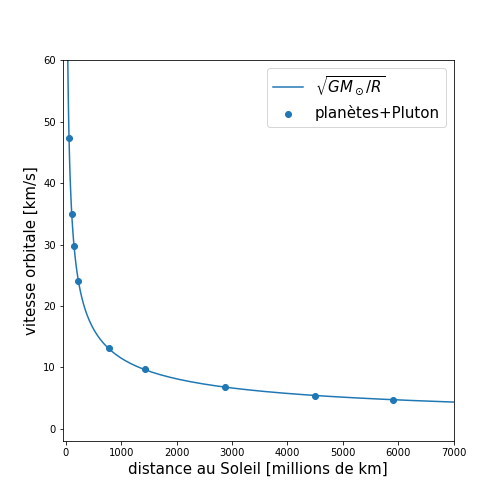
\includegraphics[height=20cm]{figs/sysol.png}
	\caption[La vitesse de rotation des planètes du système solaire]{La vitesse de rotation des planètes du système solaire + Pluton en fonction de leur distance au Soleil~: les points indiquent ces quantités pour les 9 corps en orbite autour du Soleil tandis que la ligne trace la vitesse attendue en fonction du rayon, compte tenue de la masse du Soleil. On obtient un comportement classique en $1/\sqrt{r}$.} 
	\label{f:sysol}
\end{figure}


Pour un système étendu avec un profil de masse la relation reste inchangée:
\begin{equation}
V_r(r)=\sqrt{\frac{GM(<r)}{r}}.
\end{equation}
C'est la masse comprise à l'intérieur de l'orbite qui rentre en jeu : celle-ci peut augmenter avec le rayon\sidenote{par exemple un système de densité homogène voit $M(<r)\sim r^3$  et donc $V_r\sim r$ }, mais si il existe une distance au delà de laquelle cette masse ne varie plus \sidenote{comme attendu pour un système de taille finie}, on retrouve la décroissance standard en $1/\sqrt{r}$ de la vitesse de rotation.

On peut faire le même exercice dans une galaxie ou dans la Voie Lactée\index{Voie Lactée}, en mesurant la vitesse de rotation des étoiles ou de la composante gazeuse du disque. Le résultat obtenu pour la Voie Lactée est présenté dans la figure \ref{f:rotcurve} : ce que l'on constate aisément c'est l'absence de décrochage de la vitesse de rotation dans la Galaxie et le maintien d'une vitesse constante, de l'ordre de 200 km/s, quelle que soit la distance considérée et ceci bien au delà de la limite du disque galactique (de l'ordre de 10 kpc). Ce type de courbe de rotation\index{courbe de rotation} plate est représentatif de la cinématique d'un grand nombre de galaxies de type disque dans l'Univers et indique que la distribution de la matière ne s'arrête pas aux limites du disque galactique mais s'étend au delà \sidenote{c'est l'interprétation la plus standard, d'autres possibilités sont discutées en fin de chapitre}. Cette matière est invisible, plus étendue que la matière visible et permet le maintien de vitesses de rotation importantes de par son influence gravitationnelle : cette masse supplémentaire est nommée \textit{matière noire}\index{matière noire}.

\begin{figure}[htbp]
	\centering
		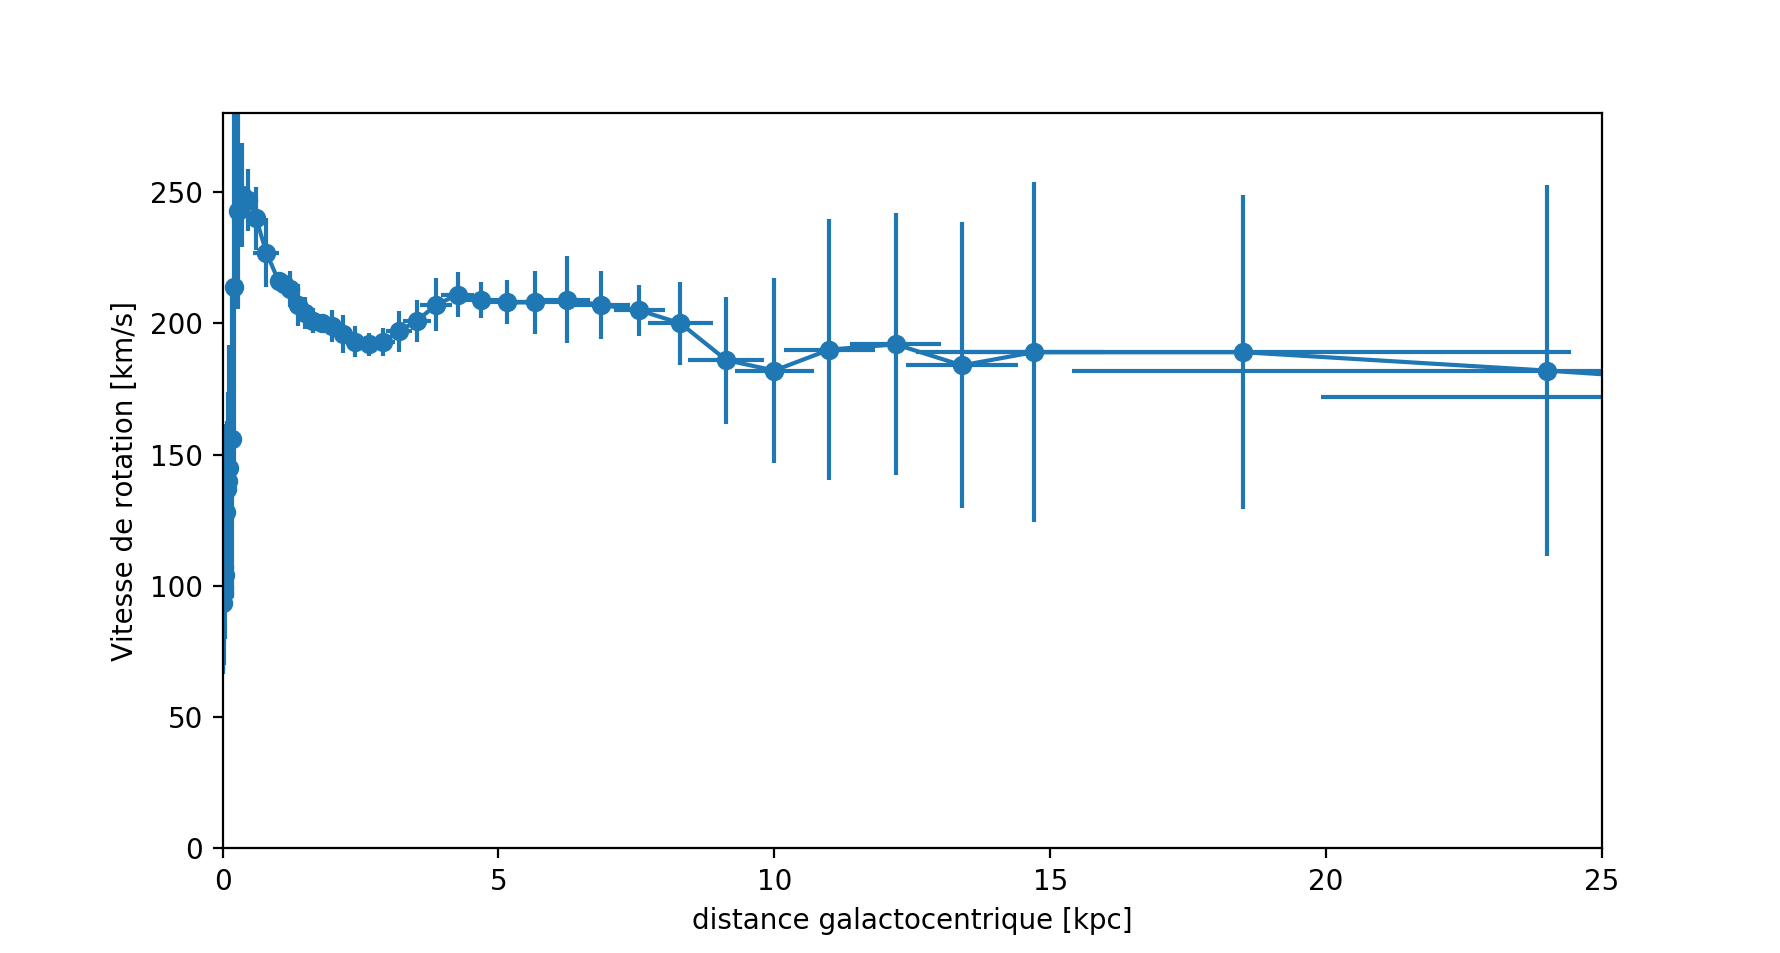
\includegraphics[height=20cm]{figs/rocurveMW.png}
	\caption[La vitesse de rotation de la matière dans la Voie Lactée]{La vitesse de rotation de la matière dans la Voie Lactée en fonction de sa distance au centre, avec leurs incertitudes. Les points de données sont issus de Sofue (2013). Cette \textit{courbe de rotation} plate est représentative de la cinématique de la très grande majorité des galaxies de type disque dans l'Univers.} 
	\label{f:rotcurve}
\end{figure}

Un calcul rapide nous indique une masse dynamique\index{masse dynamique} pour la Voie Lactée de quelques $10^{11} M_\odot$, tandis que l'on estime la masse lumineuse (étoiles + gaz) à environ 10 fois moins: non seulement la cinématique oblige à considérer une masse supplémentaire invisible mais sa contribution se doit d'être dominante.

\subsection{Amas de galaxies \index{amas de galaxies} et théorème du viriel\index{théorème du viriel}}

Les galaxies de type disques ne sont pas les seules à présenter un désaccord entre la quantité de matière estimée par la production lumineuse et les sondes dynamiques. Historiquement\sidenote{dès 1933, par Zwicky} ce type de désaccord a d'abord été mis en évidence dans les amas de galaxies\index{amas de galaxies} : ces structures dont la taille typique est de l'ordre du Mégaparsec\sidenote{donc environ 100 fois plus grandes que les galaxies} sont les plus grandes ayant pu se former au cours des 13 milliards d'années d'âge de l'Univers et peuvent contenir plusieurs centaines de galaxies.

Chacune de ces galaxies est animée d'une vitesse propre permettant d'estimer la dispersion de vitesse $\sigma$ au sein de tels amas. Dans une situation d'équilibre, cette dispersion de vitesse\index{vitesse!dispersion} est directement reliée à la masse totale du système. En effet, soit un système de N particules en interaction gravitationnelle\sidenote{chaque particule représente une galaxie de notre amas}, la particule $i$ obéit au principe fondamental de la dynamique\index{principe fondamental de la dynamique}
\begin{equation}
m_i\frac{d^2 \vec{r_i}}{dt^2}=-\sum_{j\neq i}^N \frac{Gm_i m_j (\vec{r_i}-\vec{r_j})}{||\vec{r_i}-\vec{r_j}||^3}.
\end{equation}
Cette relation est satisfaite pour toutes les particules. Multiplions-la par $\vec{r_i}$ et additionnons toutes ces relations\sidenote{le passage de la 1ère à la 2ème ligne s'obtient en considérant la double somme comme la somme des deux parties triangulaires identiques au signe près d'une matrice NxN de diagonale nulle} :
\begin{eqnarray}
\sum_i^N m_i\vec{r_i}\cdot\frac{d^2 \vec{r_i}}{dt^2}&=&-\sum_i^N \sum_{j\neq i}^N \frac{Gm_i m_j \vec{r_i}\cdot (\vec{r_i}-\vec{r_j})}{||\vec{r_i}-\vec{r_j}||^3}\\
&=& -\sum_i^N \sum_j^{i-1}\frac{Gm_i m_j}{||\vec{r_i}-\vec{r_j}||}\\
&=&E_{p,\mathrm{total}}.
\end{eqnarray}
On obtient l'énergie potentielle\index{energie@énergie potentielle} totale du système, définie comme étant la somme de toutes les énergies potentielles crées par les paires individuelles, sans redondance. Le terme de gauche peut se réécrire sous la forme:
\begin{eqnarray}
\sum_i^N m_i\vec{r_i}\cdot\frac{d^2 \vec{r_i}}{dt^2}&=&\frac{d^2}{dt^2}\sum_i^N m_i \vec{r_i}^2 - \sum_i^N m_i \left(\frac{d \vec{r_i}}{dt}\right)^2\\
&=&\frac{d^2}{dt^2}\sum_i^N m_i \vec{r_i}^2 - 2E_{c,\mathrm{total}}.
\end{eqnarray}
On reconnaît l'énergie cinétique\index{energie@énergie cinétique} totale du système ainsi que la dérivée seconde du tenseur d'inertie\index{tenseur d'inertie} par rapport au temps\sidenote{plus précisément la dérivée de la trace du tenseur d'inertie}. Cette dernière quantité décrit la 'forme' du système : à l'équilibre la répartition des masses au sein du système doit rester constante et la dérivée du tenseur d'inertie doit être nulle. On obtient alors une expression du théorème du viriel\index{théorème du viriel}
\begin{equation}
2E_{c,\mathrm{total}} + E_{p,\mathrm{total}} =0.
\end{equation}
Cette relation obtenue dans le cadre d'un système en interaction gravitationnelle n'est qu'une des multiples déclinaisons de ce théorème, que l'on retrouve dans de multiples contextes ayant trait à des systèmes à l'équilibre, en thermodynamique ou même dans le cadre de la mécanique quantique.

En supposant l'équilibre, on peut estimer la masse totale d'un système si l'on est capable d'estimer son énergie cinétique. Par exemple pour l'amas de Coma, on mesure une dispersion des vitesses $\sigma \sim 1000$ km/s pour ses galaxies membres dans un rayon d'environ 3 Mégaparsecs. Une application rapide du théorème de viriel permet d'écrire \sidenote{le facteur 3 dans l'énergie cinétique suppose une dispersion de vitesse isotrope dans les 3 directions tandis que l'énergie potentielle est celle d'un corps homogène } :
\begin{equation}
3M\sigma^2\sim \frac{3GM^2}{5R}
\end{equation}
conduisant à une estimation de sa masse de l'ordre de :
\begin{equation}
M\sim\frac{5R\sigma^2}{G}\sim 3\times 10^{15} M_\odot.
\end{equation}
Or on estime la masse lumineuse (dans les galaxies et sous la forme de gaz intra-amas) totale de l'amas de Coma à environ $1/10$ème de cette valeur. Ce désaccord entre masse dynamique et masse lumineuse est systématique dans les grands amas et illustre à nouveau le besoin d'une matière pesante non lumineuse en grande quantité.

\subsection{Halos de matière noire}

Les deux courts exemples précédents impose une image multi-phases des galaxies et des amas de galaxies: schématiquement une galaxie se compose d'une partie lumineuse composée d'étoiles, de gaz, de poussière et une partie sombre composée de matière noire. L'ajustement de modèles sur la dynamique observée des galaxies et des amas indique que cette matière est organisée en une composante plus étendue et moins dense que celle qui rayonne : les galaxies sont entourée d'un \textit{halo de matière noire}\index{matière noire!halo}. Par exemple pour une galaxie comme la Voie Lactée\index{Voie Lactée}, la masse de son halo est de l'ordre de $10^{11}-10^{12} M_\odot$ et son étendue est de l'ordre de quelques centaines de kiloparsecs. Rappelons qu'a proximité se trouve la galaxie d'Andromède légèrement plus massive et à une distance de 800 kiloparsecs environ : compte tenu de la faible séparation entre ces 2 objets, il est probable que les halos de ces 2 galaxies soient en contact.

\begin{figure}[htbp]
	\centering
		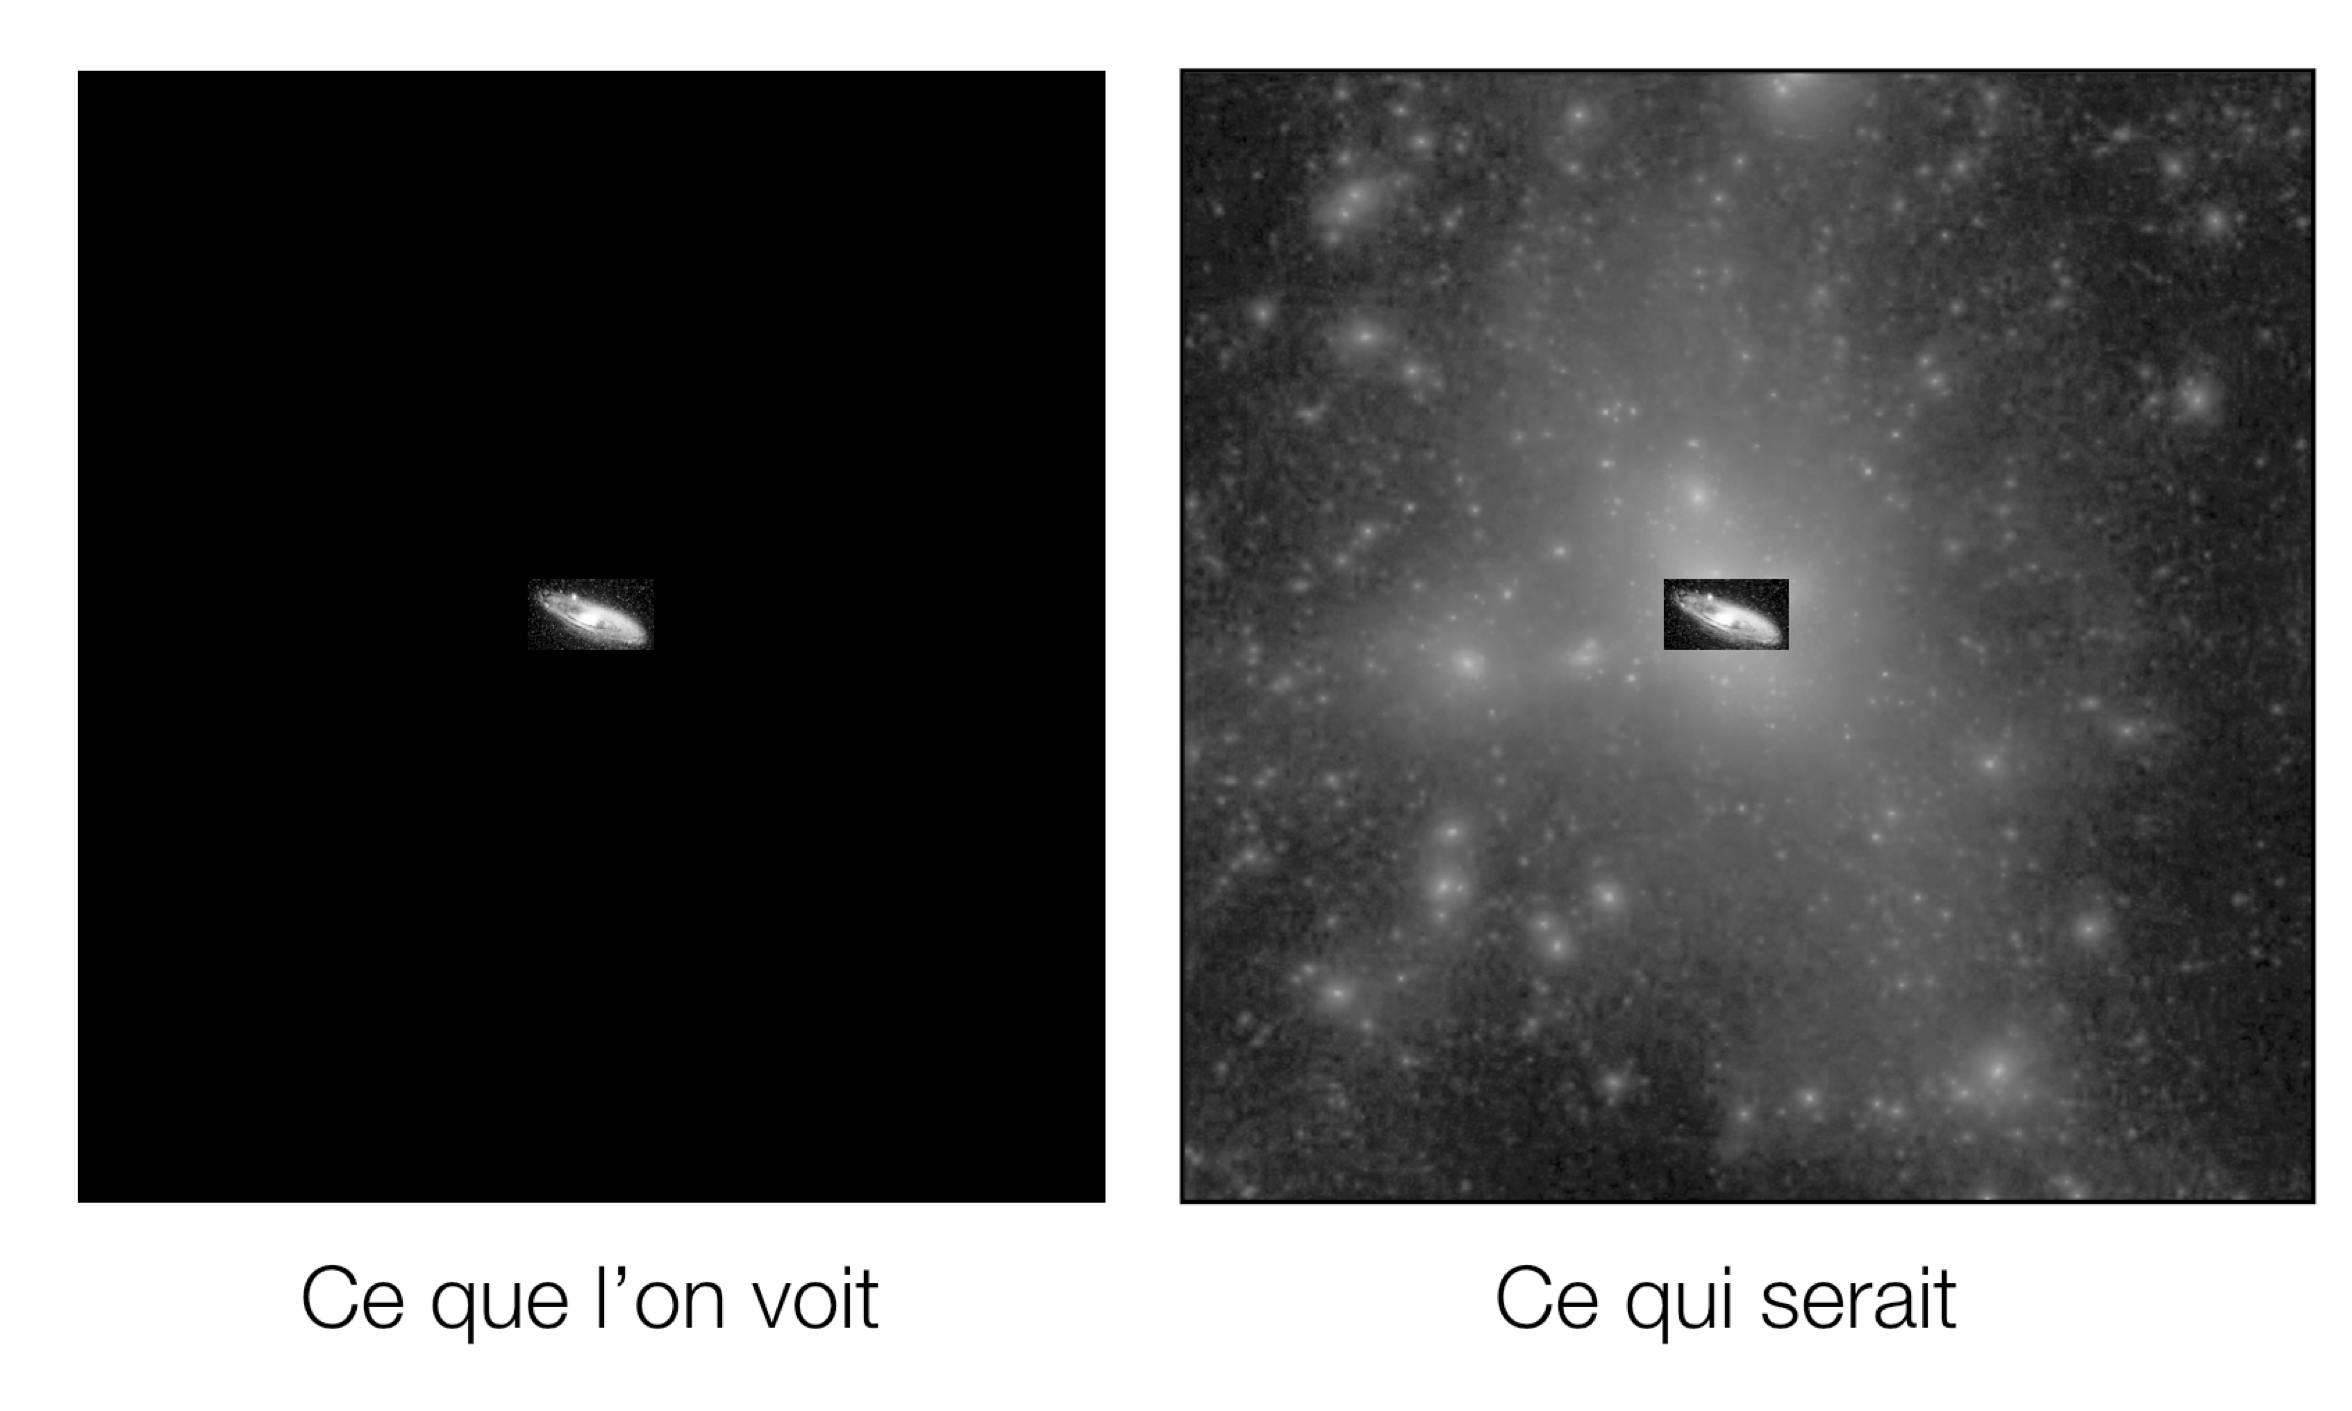
\includegraphics[height=12cm]{figs/halogal.png}
	\caption[Une galaxie et son halo de matière noire]{Vue schématique d'une galaxie et de son halo de matière noire. A gauche la partie lumineuse d'une galaxie, a droite la galaxie avec son halo de matière noire environnant (issue d'une prédiction de simulation numérique), invisible et représentant environ 90\% de sa masse totale. La figure n'est pas tout à fait à l'échelle puisque les modèles prédisent des halos de matière noire environ une dizaine de fois plus étendus que les galaxies qu'ils hébergent.} 
	\label{f:halogal}
\end{figure}


Le rapport de masse entre la composante lumineuse et noire est d'environ $1/10$ème en défaveur de la matière lumineuse. Ce chiffre n'est pas si étonnant si l'on considère le rapport cosmique de la densité d'énergie de la masse baryonique et de la masse totale :
\begin{equation}
f_b=\Omega_b/\Omega_m\sim0.15.
\end{equation}
Ce rapport est appelé \textit{la fraction baryonique}\index{fraction baryonique} on retrouve le même ordre de grandeur que celui estimé précédemment. Pour l'essentiel, galaxies et amas ne font que conserver ce rapport universel. Ce n'est toutefois pas le cas des galaxies de très faible masse ($<10^{10} M_\odot$)\sidenote{par exemple la petite galaxie de \textit{Draco} possède une masse totale environ 400 fois supérieure à ce qui est attendu compte tenu de sa luminosité} : les modèles et les observations indiquent des fractions baryoniques plus faibles que la fraction universelle pour ces objets qui ne parviennent pas à piéger le gaz de façon aussi efficace que les structures plus massives . 
\begin{figure}[htbp]
	\centering
		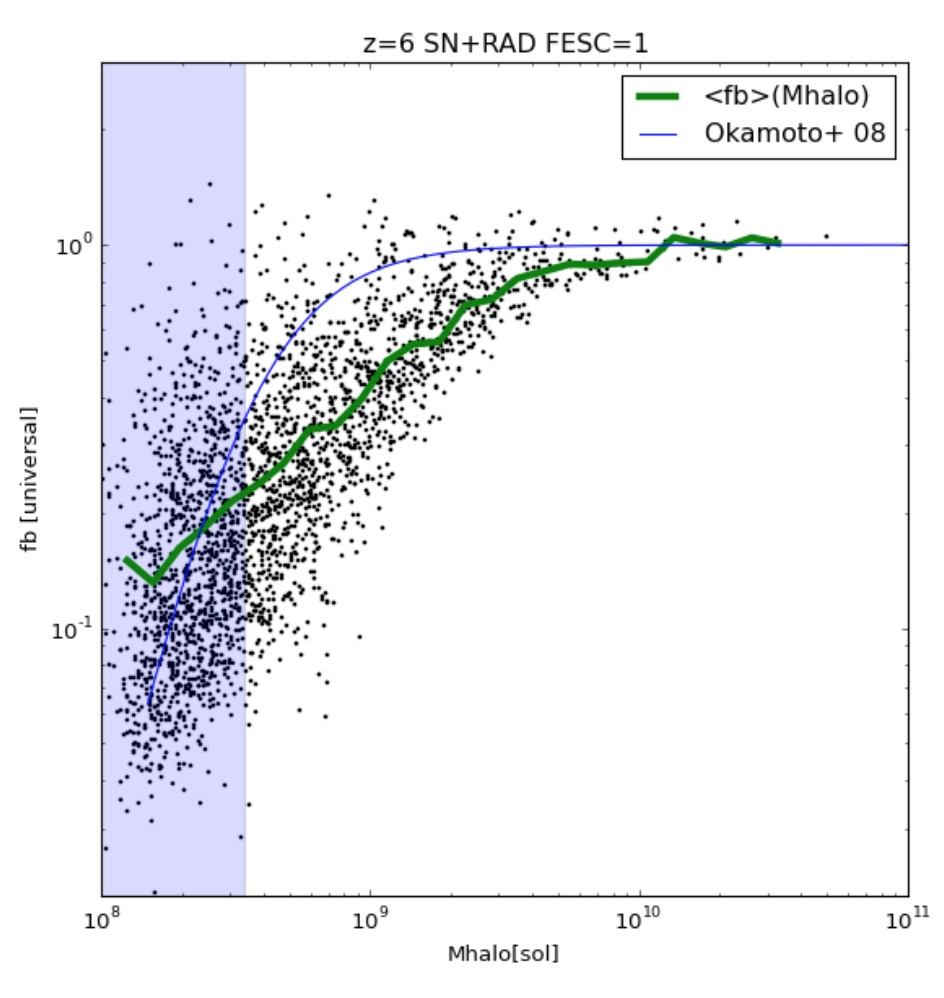
\includegraphics[height=8cm]{figs/fbar.png}
	\caption[La fraction baryonique prédite par une simulation numérique]{La fraction baryonique prédite par une simulation numérique (points) et par un modèle de Okamoto+08 (ligne) environ 1 milliards d'années après le Big-Bang. On note le départ de cette fraction à la valeur universelle pour les objets de petite masse.} 
	\label{f:fbar}
\end{figure}
Ces petits objets sont particulièrement sensibles aux effets astrophysiques tels que l'éjection de gaz par l'explosion d'étoiles en supernovæ\index{supernovae} ou le chauffage par le fond de rayonnement UV cosmique\index{fond UV} \sidenote{cf. le chapitre simulation}. Ils sont fortement dominés par la matière noire et sont donc des lieux idéaux pour l'étude de ses propriétés.

\section{Matière Non-Collisionnelle}
On sait peu de choses sur la matière noire, si ce n'est qu'elle n'interagit pas avec le champ électromagnétique (par définition) et ne ressent que la force de gravitation. Par conséquent, un ensemble de particules de matière noire se comporte de façon similaire à un ensemble d'étoiles en interactions mutuelles et tous les outils de la dynamique des systèmes stellaires peut s'appliquer à un système composé de matière noire.

Ces systèmes dont la cohésion et la dynamique sont régies par la gravitation partagent la particularité d'être \textit{non collisionnels}\index{système non collisionnel}. La non collisionalité est une propriété assez générique des systèmes auto-gravitant \sidenote{car il existe des exceptions, comme les amas stellaires dits globulaires\index{amas globulaire} qui peuplent les halos stellaires des galaxies et qui ne rentrent pas dans le cadre qui nous intéresse ici} et dont on peut saisir la nature par un examen de l'équation de Poisson\index{equation@équation!Poisson} \sidenote{$\phi$ désigne le potentiel gravitationnel\index{potentiel gravitationnel} tandis que $\rho$ désigne le champ de densité de matière } :
\begin{equation}
\frac{d^2\phi}{d\vec{r}^2}=4\pi G\rho(\vec{r}).
\end{equation} 
Cette équation constitue l'équation de champ de la gravitation newtonienne et décrit explicitement la densité comme étant la dérivée seconde du potentiel. Cette relation n'est pas sans conséquences sur la forme du potentiel : une telle relation implique que le potentiel est une version \textit{lissée} de la densité. En effet, la dérivée seconde d'une fonction quelconque est toujours plus 'bruitée' que la fonction d'origine. On peut aussi s'en rendre compte en prenant la transformée de Fourier\index{transformée de Fourier} de l'équation de Poisson pour trouver la relation entre un mode de fréquence $k=2\pi/\lambda$ du potentiel et celui de la densité\sidenote{si $\tilde f(k)$ est la transformée de Fourier de $f(x)$, on rappelle que $\tilde{f'}(k)=ik\tilde f(k)$}:
\begin{equation}
-k^2 \phi_k=4\pi G \rho_k.
\end{equation}
La relation gagne en simplicité en devenant scalaire et on constate que chaque mode de densité est \textit{amplifié} d'un facteur $k^2$ et cette amplification est d'autant plus forte que $k$ est grand: le poids des modes à grande fréquence spatiale va s'en trouver augmenté par rapport à ceux aux basses fréquences et le signal de la densité est plus bruité que celui du potentiel. Inversement, le potentiel est une version lissée de la densité de matière.
\begin{figure}[htbp]
	\centering
		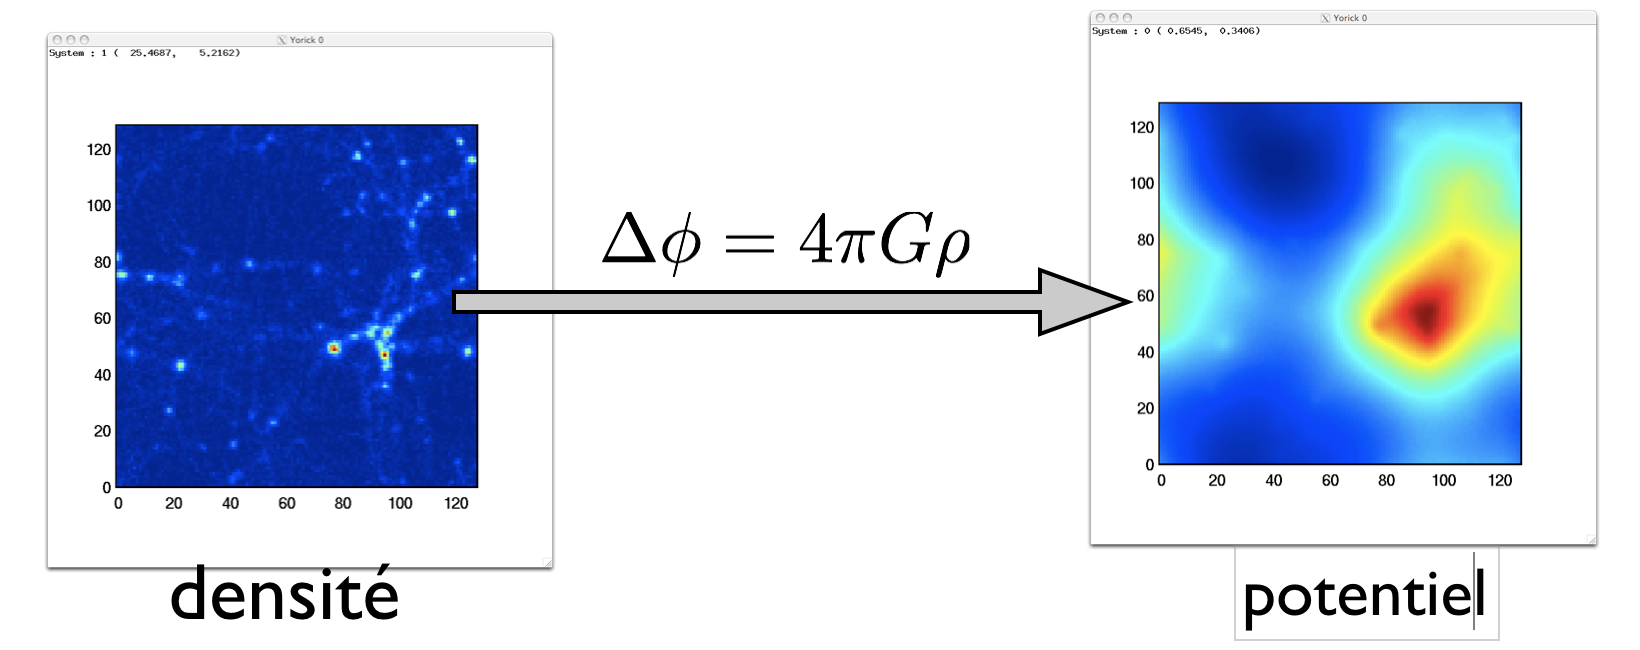
\includegraphics[height=8cm]{figs/poisson.png}
	\caption[Une illustration du lien entre densité et potentiel, via l'équation de Poisson.]{Une illustration du lien entre densité et potentiel, via l'équation de Poisson. La vignette de gauche montre la densité de matière dans une simulation cosmologique de 12 Mpc de côté, celle de droite montre la carte du potentiel gravitationnel produite par cette densité. Le potentiel est une version filtrée de la densité.} 
	\label{f:poisson}
\end{figure}

Le potentiel étant lisse, la dynamique ressentie par une particule de matière noire est sensible aux grandes échelles et non pas aux aspérités locales du champ de densité. La trajectoire d'une particule parmi ses semblables ne sera pas heurtée (comme elle le serait si elle était l'objet de \textit{collisions}) mais tendue et sans à-coups. On parle de système non-collisionnel\index{système non-collisionnel}.

On peut avoir une estimation un peu plus quantitative de cette non-collisionnalité. Considérons d'abord un système de N particules chacune de taille $r$. La section efficace d'interaction directe est $\sigma=4\pi r^2$. Le libre parcours-moyen\index{libre parcours moyen}\sidenote{la distance parcourue entre 2 interactions, qui est d'autant plus courte que les interactions sont fortes ($\sigma$ élevé) ou les densités importantes ($n$ élevé)} est donné par :
\begin{equation}
\lambda=\frac{1}{n\sigma}=\frac{4\pi R^3}{3 N \sigma}
\end{equation}
où $R$ désigne la taille du système. Si la vitesse typique d'une particule est $v$, le temps entre 2 collisions\index{temps!de collision} est donné par :
\begin{equation}
t_c=\frac{\lambda}{v}=\left(\frac{R}{r}\right)^2 \frac{t_\mathrm{crois}}{N}
\label{e:tc}
\end{equation}
où le temps de croisement $t_\mathrm{crois}=R/v$\index{temps!de croisement} est la durée nécessaire pour traverser le système. Pour un 'gaz d'étoiles' comme la Voie Lactée on a $t_c\sim 10^{21}$ ans\sidenote{on peut prendre $R=10$ kpc, $v\sim 200$ km/s, $r\sim 700 000$ km comme rayon solaire et $N\sim 10^{10}$. } : comme ce temps est très supérieur à l'âge de l'Univers, il n'y a pas de collisions entre étoiles dans un système comme la Voie Lactée. Pour la matière noire, à priori faite de particules élémentaires très nombreuses, le temps de collision est encore plus grand.
Bien sûr, cela concerne uniquement les collisions directes et il faut également prendre en compte les interaction à grande distance qui sont susceptibles de modifier la trajectoire des particules massives via la gravitation. De fait on peut montrer qu'il suffit qu'une étoile passe à une distance $b$ donnée par \sidenote{la deuxième équivalence s'obtient en appliquant le théorème du viriel}:
\begin{equation}
b\sim\frac{2Gm}{v^2}\sim R/N
\end{equation}
pour que la variation de vitesse induite par la gravitation soit du même ordre que la vitesse $v$ elle même. Cette quantité est un paramètre d'impact\index{paramètre d'impact} qui augmente avec la vitesse~: des étoiles rapides nécessitent des approches à courte distance pour ressentir une déviation substantielle, tandis que des étoiles lentes se font plus facilement perturber à plus grande distance. Si l'on remplace $r$ par $b$ dans l'expression du temps de collision (Eq. \ref{e:tc}), on obtient une estimation du temps entre 2 interactions de ce type:
\begin{equation}
t_b=\left(\frac{R}{b}\right)^2 \frac{t_\mathrm{crois}}{N}\sim N t_\mathrm{crois}.
\end{equation}
Pour une galaxie comme la Voie Lactée, $t_\mathrm{crois}$ est de l'ordre de $10^8$ ans, donc ce temps $t_b$ reste toujours extrêmement long. Enfin, on peut également refaire cette évaluation en ne considérant pas une seule interaction à une distance $b$ mais toutes les interactions plus faibles mais plus nombreuses qui se produisent à une distance comprise entre $b$ (le cas le plus intense) et $R$ (la plus grande distance possible entre une particule et sa voisine). Le temps nécessaire pour que cela conduise à une variation de vitesse équivalente à la vitesse typique est appelé \textit{temps de relaxation}\index{temps!de relaxation} et il est légèrement plus court que le précédent:
\begin{equation}
t_\mathrm{relax}=\frac{N}{10\log N} t_\mathrm{crois}.
\end{equation}
Pour une Voie Lactée on obtient $t_\mathrm{relax} \sim 10^{15}$ ans pour sa composante stellaire: cela reste largement supérieur à l'age de l'Univers et les étoiles n'ont pas perdu la mémoire de leur vitesses initiales, le système est non-collisionnel. Comme les particules de matière noire sont supposées bien plus nombreuses que les étoiles, la même conclusion s'impose à cette composante et la matière noire est non-collisionnelle.

Cela n'est pas sans conséquence sur la dynamique interne des halos de matière noire. A cause de la non-collisionnalité, les temps de mélange sont extrêmement longs et bien moins efficaces que les mélanges hydrodynamiques qui opèrent dans le gaz par exemple. On s'attend par exemple à ce que les structures de matière noire\index{matière noire} persistent sur des temps longs ou bien qu'elle puissent se croiser lors de fusions sans trop de dégâts. Les baryons (présents sous forme de gaz) possèdent une pression qui est la manifestation macroscopique de collisions microscopiques\sidenote{qui découlent de l'interaction électromagnétique entre atomes ou molécules} : cette composante peut présenter des chocs hydrodynamiques et se mélanger fort efficacement. Compte tenu de sa nature non-collisionnelle, ce n'est pas ce qui est attendu de la part de la matière noire.


\begin{figure}[htbp]
	\centering
		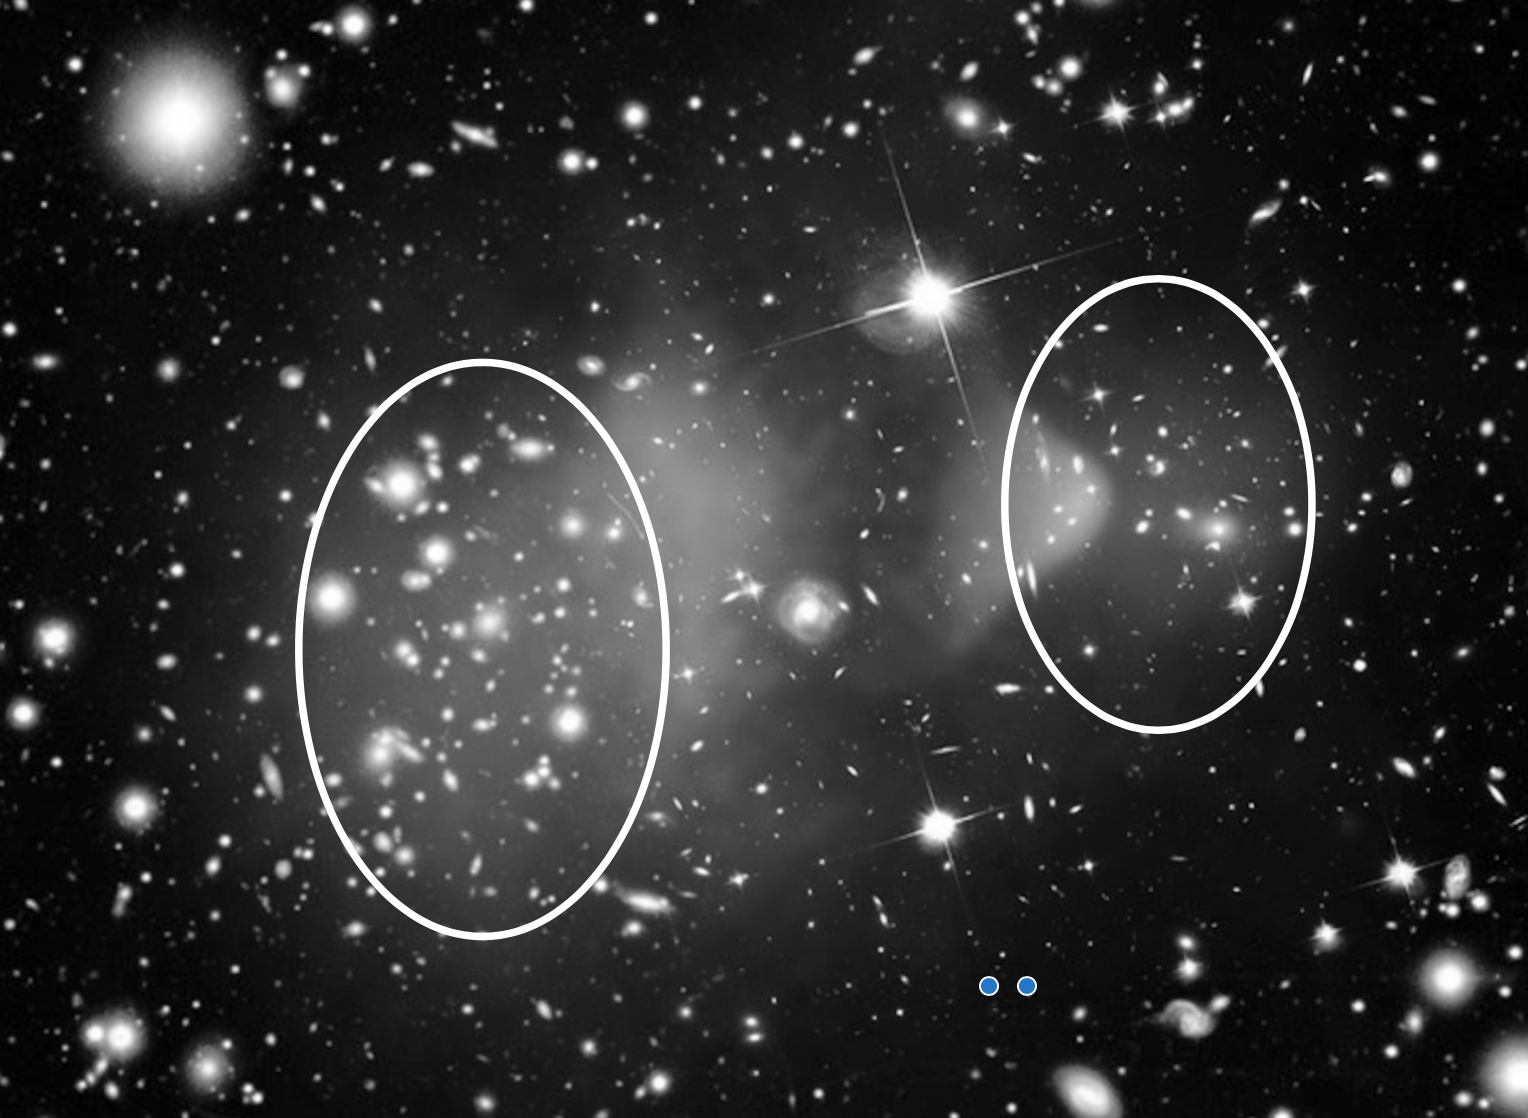
\includegraphics[height=10cm]{figs/bullet.png}
	\caption[Le \textit{Bullet Cluster}]{Le \textit{Bullet Cluster}. Cette image superpose l'image optique de 2 amas en collisions, la carte de la distribution de masse et la carte de la distribution de gaz. On distingue parfaitement le choc hydrodynamique de forme triangulaire dû à la collision. Les ellipses indiquent la position de la masse dominante, mesurée via les effets de lentilles gravitationnelles. On constate que les ellipses sont décalées par rapport au gaz comme attendu pour la matière noire non collisionnelle. Figure inspirée de l'image NASA (M. Markevitch et al.;  D.Clowe et al.).} 
	\label{f:bullet}
\end{figure}

Cette différence de comportement a peut-être été observée dans le \textit{Bullet cluster}\index{Bullet cluster} présenté dans la Figure \ref{f:bullet}. C'est une région du ciel dans laquelle 2 amas de galaxies sont entrés en collision. On y a superposé la distribution de gaz (sondée par son rayonnement X) et la distribution de masse totale (gaz+autre). On distingue aisément dans la composante gazeuse le choc hydrodynamique\index{choc} dû à la collision avec une forme en arc caractéristique. On constate également aisément que la masse n'est pas superposée à l'émission du gaz, comme si l'essentiel de la masse avait pu parcourir une distance plus grande que celle des baryons lors du choc : c'est exactement le comportement attendu pour la matière noire non-collisionnelle dont on rappelle qu'elle doit dominer largement le bilan en masse. Lors de leur collision, la partie gazeuse des 2 amas a choqué et freiné tandis que la composante matière noire\index{matière noire} non collisionnelle a pu poursuivre sa route et se découpler des baryons. 

\subsection{Lentilles gravitationnelles\index{lentille gravitationnelle}}
Nous venons de mentionner que la masse totale du Bullet Cluster ne présente pas la même distribution que celle de la masse baryonique : mais au fait comment fait-on pour trouver la distribution de masse totale? La réponse se trouve dans l'utilisation de l'effet de \textit{lentilles gravitationnelles}\index{lentille gravitationnelle}. Ce terme désigne les déformations créées par un objet massif sur la trajectoire des rayons lumineux émis par des objets d'arrière-plan~: ces déformations vont induire une modification de la perception de ces objets de fond.

Il existe toute une littérature dédiée à ce phénomène, nous allons ici présenter rapidement quelques bases dans le régime simple des lentilles minces. On considère 2 plans à 2 dimensions : le plan source où se trouve les objets d'arrière-plan sur le ciel et à l'intérieur duquel les positions sont déterminées à l'aide d'un vecteur 2D $\vec{\beta}$, et le plan de la lentille, à l'intérieur duquel les déflections des rayons lumineux vont avoir lieu et où les positions sont déterminées à l'aide d'un autre vecteur 2D sur le ciel $\vec{\theta}$. Une image à la position $\vec{\theta}$ peut être reliée à un point du plan source via \textit{l'équation des lentilles}\index{equation@équation!des lentilles}
\begin{equation}
\vec{\beta}(\vec{\theta})=\vec{\theta}-\vec{\alpha}(\vec{\theta}).
\end{equation}
Ici $\vec{\alpha}(\vec{\theta})$ désigne l'angle de déflection\index{lentilles gravitationnelles!angle de déflection} subi par le rayon lumineux qui tape le plan de la lentille à cette position~: cet angle est lié à la distribution de matière dans la lentille et l'étude de la déformation des images d'arrière-plan permet de remonter à cette quantité et donc à la structure de la lentille. En effet, on peut écrire l'angle de déflection comme le gradient d'un potentiel\index{lentilles gravitationnelle!potentiel} 2D de lentille $\psi(\vec{\theta})$:
\begin{equation}
\vec{\alpha}(\vec{\theta})=\nabla \psi(\vec{\theta}).
\end{equation}
Ce potentiel satisfait également un analogue à l'équation de Poisson\index{equation de Poisson@équation de Poisson!lentille gravitationnelle}
\begin{equation}
\Delta \psi(\vec{\theta}) = 2 \kappa (\vec{\theta})
\end{equation}
où $\kappa (\vec{\theta})$ s'appelle la convergence\index{lentilles gravitationnelle!convergence} : cette quantité mesure la déformation isotrope des sources de fond et est directement reliée à la densité de matière 2D projetée $\Sigma(\vec{\theta})$\sidenote[][-3cm]{Ici $\Sigma_c$ désigne une densité surfacique 'critique'\index{lentilles gravitationnelles!densité critique} qui dépend de la configuration du banc optique (distance observateur-lentille, lentille-source) ainsi que de la cosmologie}:
\begin{equation}
\kappa (\vec{\theta}) =\frac{\Sigma(\vec{\theta})}{\Sigma_c}.
\end{equation}
In fine, la mesure des déformations permet de remonter à la densité de matière projetée, via la modélisation de lentilles gravitationnelles. Le cœur de cette modélisation est le potentiel 2D projeté $\psi(\vec{\theta})$ et au vu de la relation entre l'angle de déflection et ce potentiel, $\vec{\alpha}(\vec{\theta})$ apparaît comme l'analogue du champ de 'force' 2D. Au passage, le fait que l'on travaille à 2 dimensions n'est pas sans conséquences~: par exemple une masse projetée ponctuelle va produire un champ de déflection $\vec{\alpha}(\vec{\theta})\sim 1/\theta$ et un potentiel $\psi \sim \log \theta$. En 3D, la même masse ponctuelle aurait produit respectivement un champ de force en $1/r^2$ et un potentiel en $1/r$~: le fait de projeter les masses et par extension toutes les quantités va 'lisser' les comportement auxquels nous sommes habitués à trois dimensions.
\begin{figure}[htbp]
	\centering
		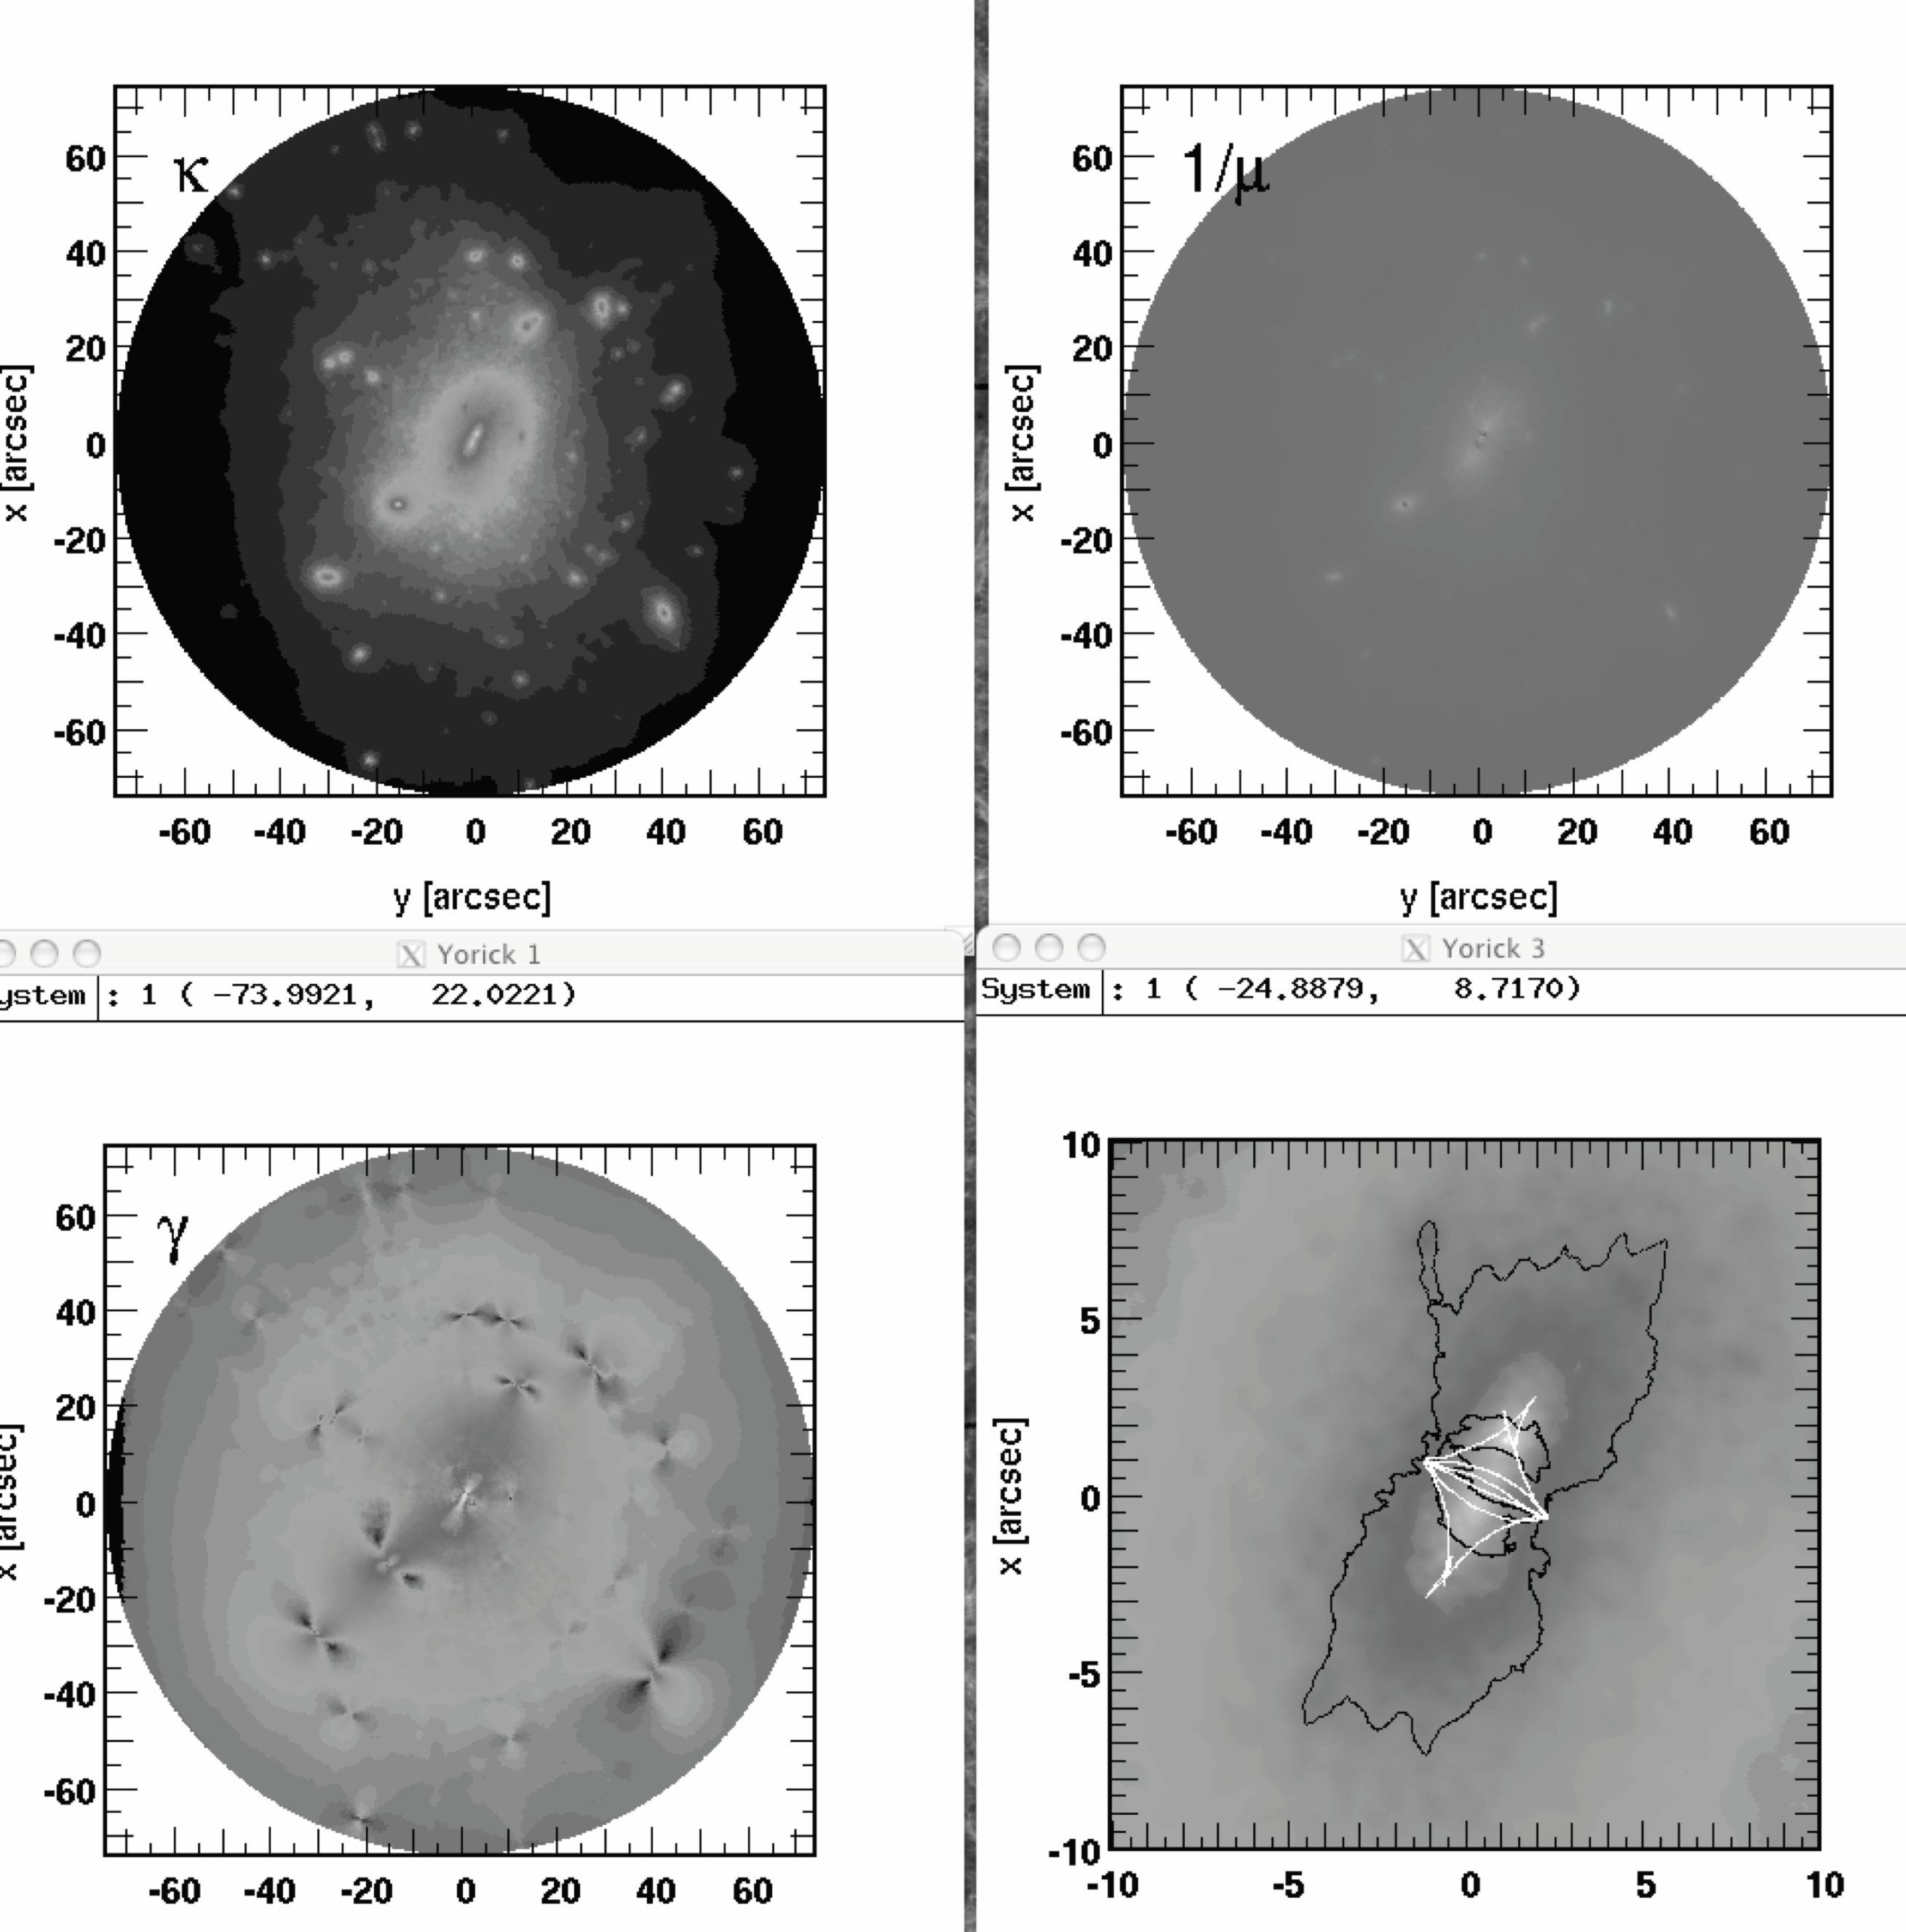
\includegraphics[height=12cm]{figs/SPLHALO.png}
	\caption[Les quantités pertinentes d'une lentille gravitationnelle]{Exemple de quantités calculées pour une lentille arbitraire. Le panneau supérieur gauche montre la densité projetée de la lentille créée par un halo de matière noire simulé, analogue à sa convergence $\kappa$. Le panneau inférieur gauche montre la distribution du cisaillement tandis que le panneau supérieur droit montre l'inverse du grossissement. Les lieux où l'inverse du grossissement est nul constituent les lignes critiques dans le plan lentille (montrées en noir sur le panneau inférieur droit) tandis que les lignes caustiques associées, dans le plan lentille, sont indiquées en blanc.} 
	\label{f:SPLHALO}
\end{figure}

On peut montrer que si la convergence est telle que $\kappa >1$ une même source peut avoir de multiples images~: on parle alors de régime de lentilles fort\sidenote{strong lensing}, le cas inverse étant celui de faibles déformations dit de lentilles faibles\sidenote{weak lensing}. Par ailleurs, on peut définir une matrice de déformation $A_{ij}=\frac{\partial \beta_i}{\partial \theta_j}$~: \textit{le grossissement} \index{lentilles gravitationnelles!grossissement}est alors donné par:
\begin{equation}
\mu(\vec{\theta})=\frac{1}{(1-\kappa(\vec{\theta}))^2 - |\vec{\gamma}(\vec{\theta})|^2}
\end{equation} 
où $\gamma$ désigne le cisaillement\sidenote{on parle de 'shear' en anglais}\index{lentilles gravitationnelles!cisaillement}, c'est à dire une mesure de la déformation anisotrope\sidenote{les 2 composantes du cisaillement sont données par $\gamma_1=(A_{11}-A_{22})/2$ et $\gamma_2=A_{12}=A_{21}$.}. On note que le grossissement\index{lentilles gravitationnelles!grossissement} peut être infini et l'ensemble des points du plan lentille où $1/\mu=0$ est appelé \textit{lignes critiques} : lorsque l'on ramène ces lignes critiques\index{lentilles gravitationnelles!lignes critiques} dans le plan source, via l'équation des lentilles, on obtient ce qu'on appelle les caustiques\index{lentilles gravitationnelles!caustiques}. A chaque fois qu'une source traverse un jeu de caustiques, son nombre d'images augmente de 2, tandis qu'une source placée exactement sur une caustique va voir son image extrêmement déformée.

\begin{figure}[htbp]
	\centering
		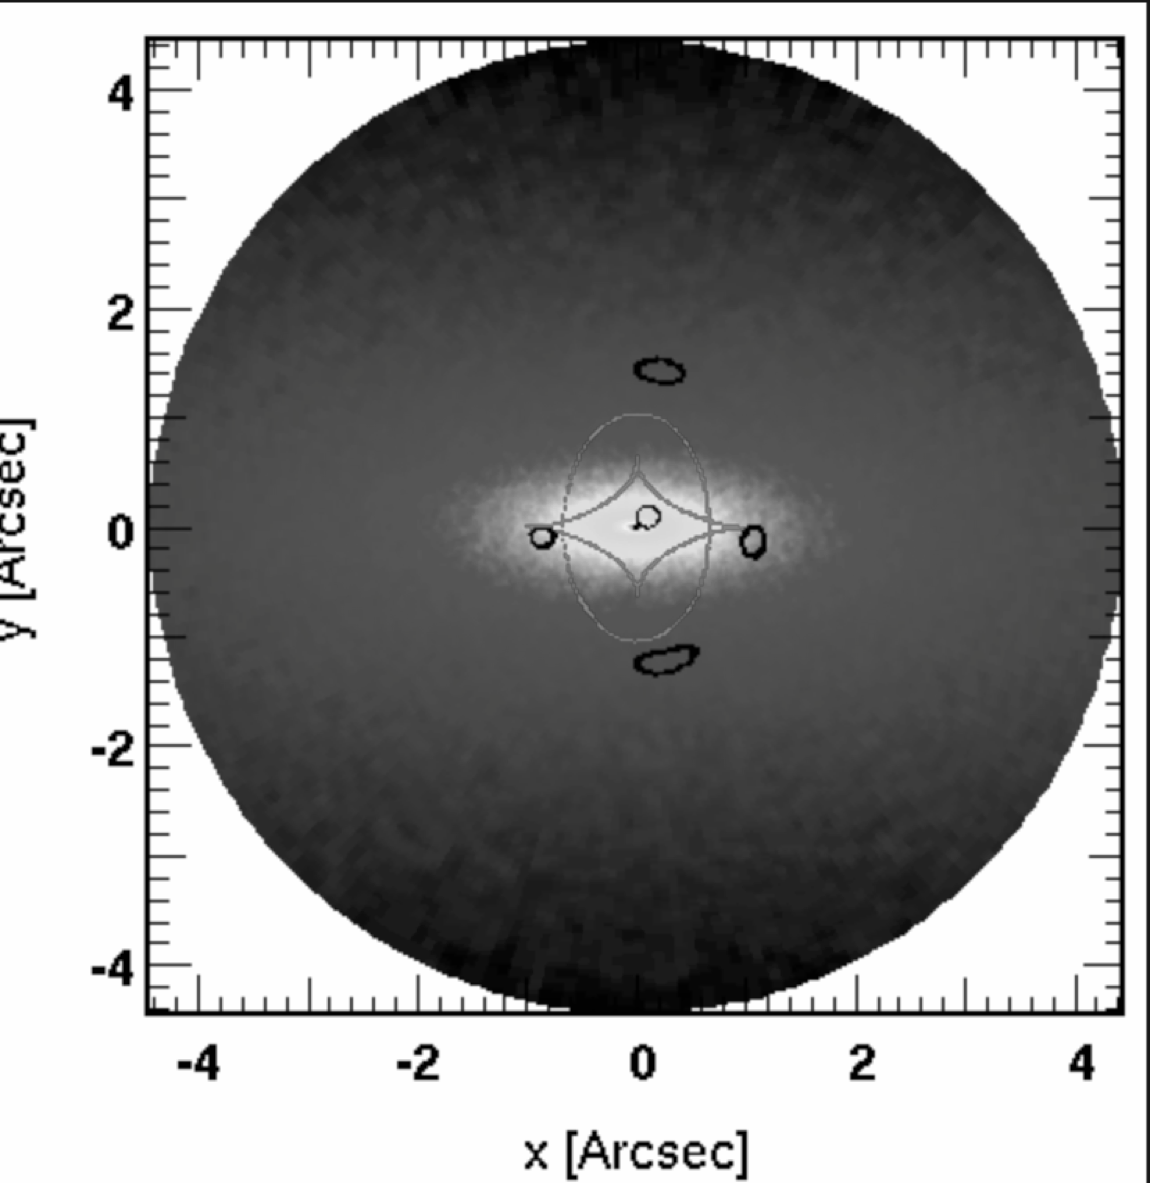
\includegraphics[height=12cm]{figs/SPL.png}
	\caption[Exemple de calcul de lentilles gravitationnelles]{Cette image montre les images produites par la source circulaire placée au quasi-centre de l'image (contours noirs). Cette source produit 5 images, les 4 situées en croix + une centrale quasi indistinguable. Les teintes de fond indiquent la distribution de matière dans une lentille elliptique, tandis que les lignes claires montrent les positions des caustiques dans le plan source. Dans ce cas précis, la source, le centre de la lentille et l'observateur sont tous quasiment alignés le long de l'axe optique.} 
	\label{f:SPL}
\end{figure}

Notons qu'il existe des configurations sources-lentilles qui donnent des images particulièrement spectaculaires. Par exemple, dans le cas d'une lentille à symétrie de révolution autour de l'axe optique, la présence d'une source d'arrière plan exactement sur cet axe conduit à un \textit{anneau d'Einstein} où la déformation de la source est telle qu'elle apparaît comme un anneau, continu, le long d'une ligne critique. Toute spectaculaire qu'elle soit, ce type de configurations est régulièrement observé dans le ciel. Si le même alignement se présente pour une lentille anisotrope (aplatie dans une direction par exemple), cet anneau se 'brise' et produit de multiples images de la source d'arrière-plan : on peut alors obtenir l'effet de 'croix d'Einstein', où chaque image se trouve aux extrémités d'une croix fictive centrée sur l'axe optique (voir figure \ref{f:SPL}).


\section{Matière noire et fond diffus cosmologique}

Les discussions précédentes ont porté sur l'influence dynamique de la matière noire sur les structures telles que les galaxies ou les amas. Il s'avère que l'évidence la plus forte quant à l'existence d'une telle matière est plutôt à trouver du côté du fond diffus cosmologique\index{fond diffus cosmologique}. Comme indiqué dans le chapitre dédié, la structure spatiale du fond diffus cosmologique trace la structure spatiale des baryons, du gaz ionisé, au moment de la Recombinaison. Cette structure révèle la présence d'ondes sonores\index{ondes sonores} parcourant le plasma à ces époques\sidenote{ces ondes sont les oscillations baryoniques acoustiques \index{oscillation baryonique acoustique} décrites à plusieurs reprise dans cet ouvrage}. Ces ondes sont supportées par la pression\index{pression!de rayonnement} de rayonnement, support autorisé par le fort couplage entre les baryons et le rayonnement avant la Recombinaison\index{Recombinaison}. Ce couplage est toutefois imparfait, les photons possèdent un libre parcours moyen non-nul qui conduit à un amortissement progressif de ces ondes, notamment celles associées aux plus petites échelles spatiales et aux plus grandes fréquences temporelles d'oscillation. Cet effet, connu sous le nom \textit{d'amortissement Silk}\index{amortissement Silk},  efface les surdensités de petites tailles et doit en principe empêcher l'émergence de structures de masse inférieure à $M\sim 10^{13} M_\odot$ : une structure comme la Voie Lactée n'aurait ainsi pas dû apparaître ! La matière noire\index{matière noire} fourni un contrepoint à cet amortissement car elle agit comme un fond de potentiel gravitationnel en effondrement continu : tandis que la distribution de gaz voit ses surdensités se faire effacer, la distribution de matière noire voit ses surdensités croître car insensibles aux effets de pression radiative et d'amortissement Silk. Au moment de la perte du support de pression radiative, les baryons trouvent un champ de gravitation plus fort que celui qu'ils auraient créé s'ils avaient étés seuls et profitent de ce champ pour faire ré-émerger des surdensités fortement amorties : le gaz 'coule' dans les puits de champ gravitationnel crées par la matière noire. 

\begin{figure}[htbp]
	\centering
		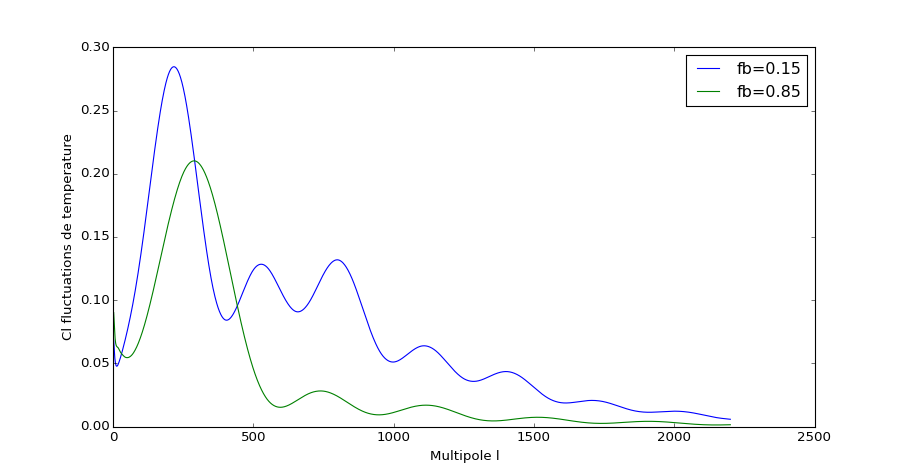
\includegraphics[height=8cm]{figs/cl_silk.png}
	\caption[Deux modèles de spectre de puissance angulaire du fond diffus cosmologique]{Deux modèles de spectre de puissance angulaire du fond diffus cosmologique. L'un possède une fraction de baryons faible, conforme au modèle standard $\Lambda CDM$, l'autre possède une fraction de baryons forte, où la contribution de la matière noire et celle des baryons est inversée par rapport au modèle standard. On note l'effet de l'amortissement Silk important aux petites échelles angulaires (grand $\ell$) dans le cas d'un Univers dominé par les baryons. A l'inverse, le modèle standard présente des pics secondaires importants traduisant l'entretien des oscillations baryoniques par le champ de gravité de la matière noire.} 
	\label{f:cl_silk}
\end{figure}

\newthought{La structure du fond diffus}, telle qu'elle est mesurée sur la surface de dernière diffusion, laisse transparaître ce rôle important de la matière noire (voir Fig. \ref{f:cl_silk}). Son spectre de puissance\index{spectre de puissance} angulaire $C_\ell$ mesuré par Planck\index{Planck!satellite} présente ainsi des pics secondaires d'amplitudes substantielles, bien plus importantes que celles qui auraient été obtenues dans une Univers avec seulement des baryons. On note en particulier la hauteur importante du troisième pic, qui est une forte indication sur la présence d'une matière non couplée par le rayonnement et qui ne subit pas d'amortissement spectaculaire. Remarquons enfin que l'amortissement Silk reste présent, mais sa force est atténuée par rapport à un modèle composé uniquement de baryons. Cette amplitude importante de pics secondaires est très difficile à expliquer sans invoquer une matière à faible interaction avec le rayonnement et de fait la structure spatiale du fond diffus cosmologique est un argument très important en faveur de l'existence de cette matière inconnue : la physique qui y opère est relativement simple, proche du régime linéaire et très bien connue au contraire de la physique plus complexe des galaxies et des amas, qui laissent plus de place à des interprétations alternatives.

\section{Matière Noire Froide}

\newthought{Le modèle standard} de la cosmologie considère également que la matière noire est \textit{froide}\index{matière noire!froide}\sidenote{en anglais on parle de CDM, \textit{Cold Dark Matter}}. Ce terme permet d'indiquer que la vitesse typique de ces particules est faible, les qualifiant de fait comme des particules non-relativistes. Le qualificatif 'froid' provient de l'analogie entre dispersion de vitesse\index{vitesse!dispersion} et température des particules dans un gaz, où l'énergie cinétique typique vaut:
\begin{equation}
m\sigma^2 \sim k_B T.
\end{equation}
Le régime non-relativiste, où $\sigma \ll c$ implique par extension une température basse et donc froide. Ce terme de matière noire froide est à mettre en opposition avec la matière noire chaude, composée de particules relativistes possédant des vitesses caractéristiques proches de celle de la lumière. Un candidat naturel à de la matière noire chaude\index{matière noire!chaude} aurait été le neutrino\index{neutrino} : cette particule interagit peu avec les autres particules, n'interagit pas avec le rayonnement, satisfaisant ainsi les qualités fondamentales de la matière noire. Le neutrino est aussi une particule très légère et relativiste, lui conférant des vitesses caractéristiques élevées et une cinématique 'chaude'\sidenote{en anglais on parle de HDM, \textit{Hot Dark Matter}}.

\subsection{Masse de Jeans : cas d'un système non-collisionel}
\newthought{Le caractère chaud} ou froid de la matière noire a des conséquences sur le type de structures que l'on peut construire avec cette matière. En effet les grandes dispersions de vitesses attendues dans le cas d'une matière noire chaude l'empêche de former des petites structures peu massives sous l'effet de la gravitation : il faut qu'une structure ait une masse suffisante pour que son 'poids' puisse s'opposer à l'effet de dispersion dû aux vitesses de particules. Cette masse critique se nomme la masse de Jeans\index{masse de Jeans}\sidenote{on la retrouvera dans une approche fluide dans le chapitre sur les grandes structures}.

L'expression de la Masse de Jeans pour un système non collisionnel peut s'obtenir en considérant l'équation qui décrit l'évolution dynamique d'un tel système, \textit{l'équation de Boltzmann}\index{equation@équation!de Boltzmann} :
\begin{equation}
\frac{d f}{dt}=\frac{\partial f}{\partial t}+\vec{\dot x}\cdot\frac{\partial f}{\partial \vec{x}}+\vec{\dot v}\frac{\partial f}{\partial \vec{v}}=0.
\end{equation}
Cette équation est juste la traduction de la conservation dans l'espace des phases de la \textit{fonction de distribution} $f(\vec{x},\vec{v},t)$\index{fonction de distribution} de notre fluide non-collisionnel. Cette fonction décrit la distribution des éléments de notre système au cours du temps, à différentes vitesses et positions. Par exemple la densité de particules  et l'impulsion à une position $\vec{x}$ sont données par :
\begin{eqnarray}
\rho(x,t)&=&\int d\vec{v} f,\\
\rho \vec{v}(x,t)&=&\int d\vec{v}\vec{v} f.
\end{eqnarray}
L'équation de Boltzmann est très générique et son intégration peut conduire par exemple à l'équation de conservation de la masse\sidenote{en intégrant sur les vitesses $\int d\vec{v}$} ou de l'impulsion \sidenote{en intégrant sur les vitesses en $\int d\vec{v} \vec{v}$}. L'absence de collisions est à l'origine du terme source égal à zéro et de la conservation de la fonction de distribution.

\newthought{Dans le régime des faibles perturbations}, on peut linéariser l'équation de Boltzmann en ne considérant que de faibles perturbations $f_1\ll f_0$ à la fonction de distribution, où $f_0(\vec{v},t)$ est la fonction de distribution homogène à l'équilibre. On obtient \sidenote{en pratique on obtient  l'équation linéarisée en injectant $f_0+f_1$ dans l'équation de Boltzmann, tout en tenant compte du fait que $f_0$ par définition satisfait sa propre équation de Boltzmann}:
\begin{equation}
\frac{\partial f_1}{\partial t}+\vec{\dot x}\cdot\frac{\partial f_1}{\partial \vec{x}}-\frac{\partial \Phi_1}{\partial \vec{x}}\frac{\partial f_0}{\partial \vec{v}}=0.
\end{equation}
Le potentiel gravitationnel\index{potentiel gravitationnel} perturbé $\Phi_1(\vec{x},t)$ apparaît en considérant le principe fondamental de la dynamique\sidenote{$\vec{\dot v}=-\vec{\nabla} \Phi_1$}.

Dans quel cas a-t-on une perturbation stable ? Intuitivement, on peut considérer que la situation est stable si $f_1$ oscille autour d'une valeur nulle. La transposition de cette intuition consiste à développer la perturbation (et le potentiel associé) comme une onde plane\sidenote{de longueur d'onde $\lambda=2\pi/k$ et de période $T=2\pi/\omega$} et considérer les conséquences de cette hypothèse au travers de l'équation de Boltzmann\index{equation@équation! de Boltzmann}
\begin{eqnarray}
f_1&=&F_1(\vec{v})e^{i(\vec{k}\vec{x}-\omega t)}\\
\Phi_1&=&P_1e^{i(\vec{k}\vec{x}-\omega t)}.
\end{eqnarray}
L'équation de Boltzmann linéarisée devient alors:
\begin{equation}
(\vec{k}\vec{v}-\omega )F_1-P_1\vec{k}\cdot\frac{\partial f_0}{\partial \vec{v}}=0
\end{equation}
Par ailleurs le potentiel satisfait l'équation de Poisson\index{equation de Poisson@équation de Poisson}\sidenote{$\Delta \Phi_1 = 4\pi G \rho$} donc la relation suivante s'applique:
\begin{equation}
-k^2 P_1=4\pi G \int d\vec{v} F_1.
\end{equation}
On obtient alors une relation de dispersion reliant la fréquence spatiale $k$ et la pulsation $\omega$ sous forme intégrale:
\begin{equation}
1+\frac{4\pi G}{k^2}\int \frac{\vec{k}\cdot\frac{\partial f_0}{\partial \vec{v}}}{\vec{k}\vec{v}-\omega}d\vec{v}=0.
\end{equation}
En principe, la résolution de cette équation doit nous permettre de dégager les solutions stables (avec $\omega$ réel)\index{stabilité} et les solutions instables\index{instabilité} (avec $\omega$ imaginaire \sidenote{qui transforme l'exponentielle complexe oscillante en exponentielle réelle croissante}). Toutefois, cette résolution est complexe et technique, en particulier du fait de la présence du terme $\vec{k}\vec{v}-\omega$ au dénominateur de l'intégrande qui rend possible l'apparition de solutions 'catastrophiques' ou résonantes. Ce type de situation est typique de la dynamique de systèmes non collisionnels et nécessite un traitement mathématique rigoureux que nous n'allons pas faire ici. Ceci étant, on peut considérer que la solution $\omega=0$ doit constituer la transition entre régime stable et instable.

\newthought{Posons $\omega=0$} et mettons nous dans le cas simple d'une fonction de distribution 'thermique'\sidenote{Maxwellienne}\index{fonction de distribution!Maxwell} à l'équilibre:
\begin{equation}
f_0(v)=\frac{\rho_0}{(2\pi\sigma^2)^{3/2}}e^{-v^2/2\sigma^2}
\end{equation}
où $\rho_0$ désigne la densité de matière moyenne et $\sigma\sim \sqrt{k_B T}$ sa dispersion de vitesse. Prenons arbitrairement le mode $\vec{k}=(k_J,0,0)$ en cartésien et l'on obtient alors\sidenote{Rappel $\frac{1}{\sqrt{2\pi \sigma^2}}\int e^{-x^2/2\sigma^2}dx=1$}:
\begin{equation}
1-\frac{4\pi G \rho_0}{k_J^2\sigma^2}=0.
\end{equation}
La transition vers le déséquilibre, donc la perte du comportement oscillant qui conduit vers l'effondrement gravitationnel, est donc caractérisée par:
\begin{equation}
\lambda_J\equiv\frac{2\pi}{k_J}=\frac{\pi \sigma}{\sqrt{G\rho_0}}.
\end{equation} 
Il existe une longueur typique $\lambda_J$ où l'onde passe dans un régime d'instabilité. C'est la longueur de \textit{Jeans}\index{longueur de Jeans} pour un système non collisionnel qui constitue la taille \textit{minimale} que doit avoir une fluctuation pour être instable et donc s'effondrer gravitationnellement.

\begin{figure}[htbp]
	\centering
		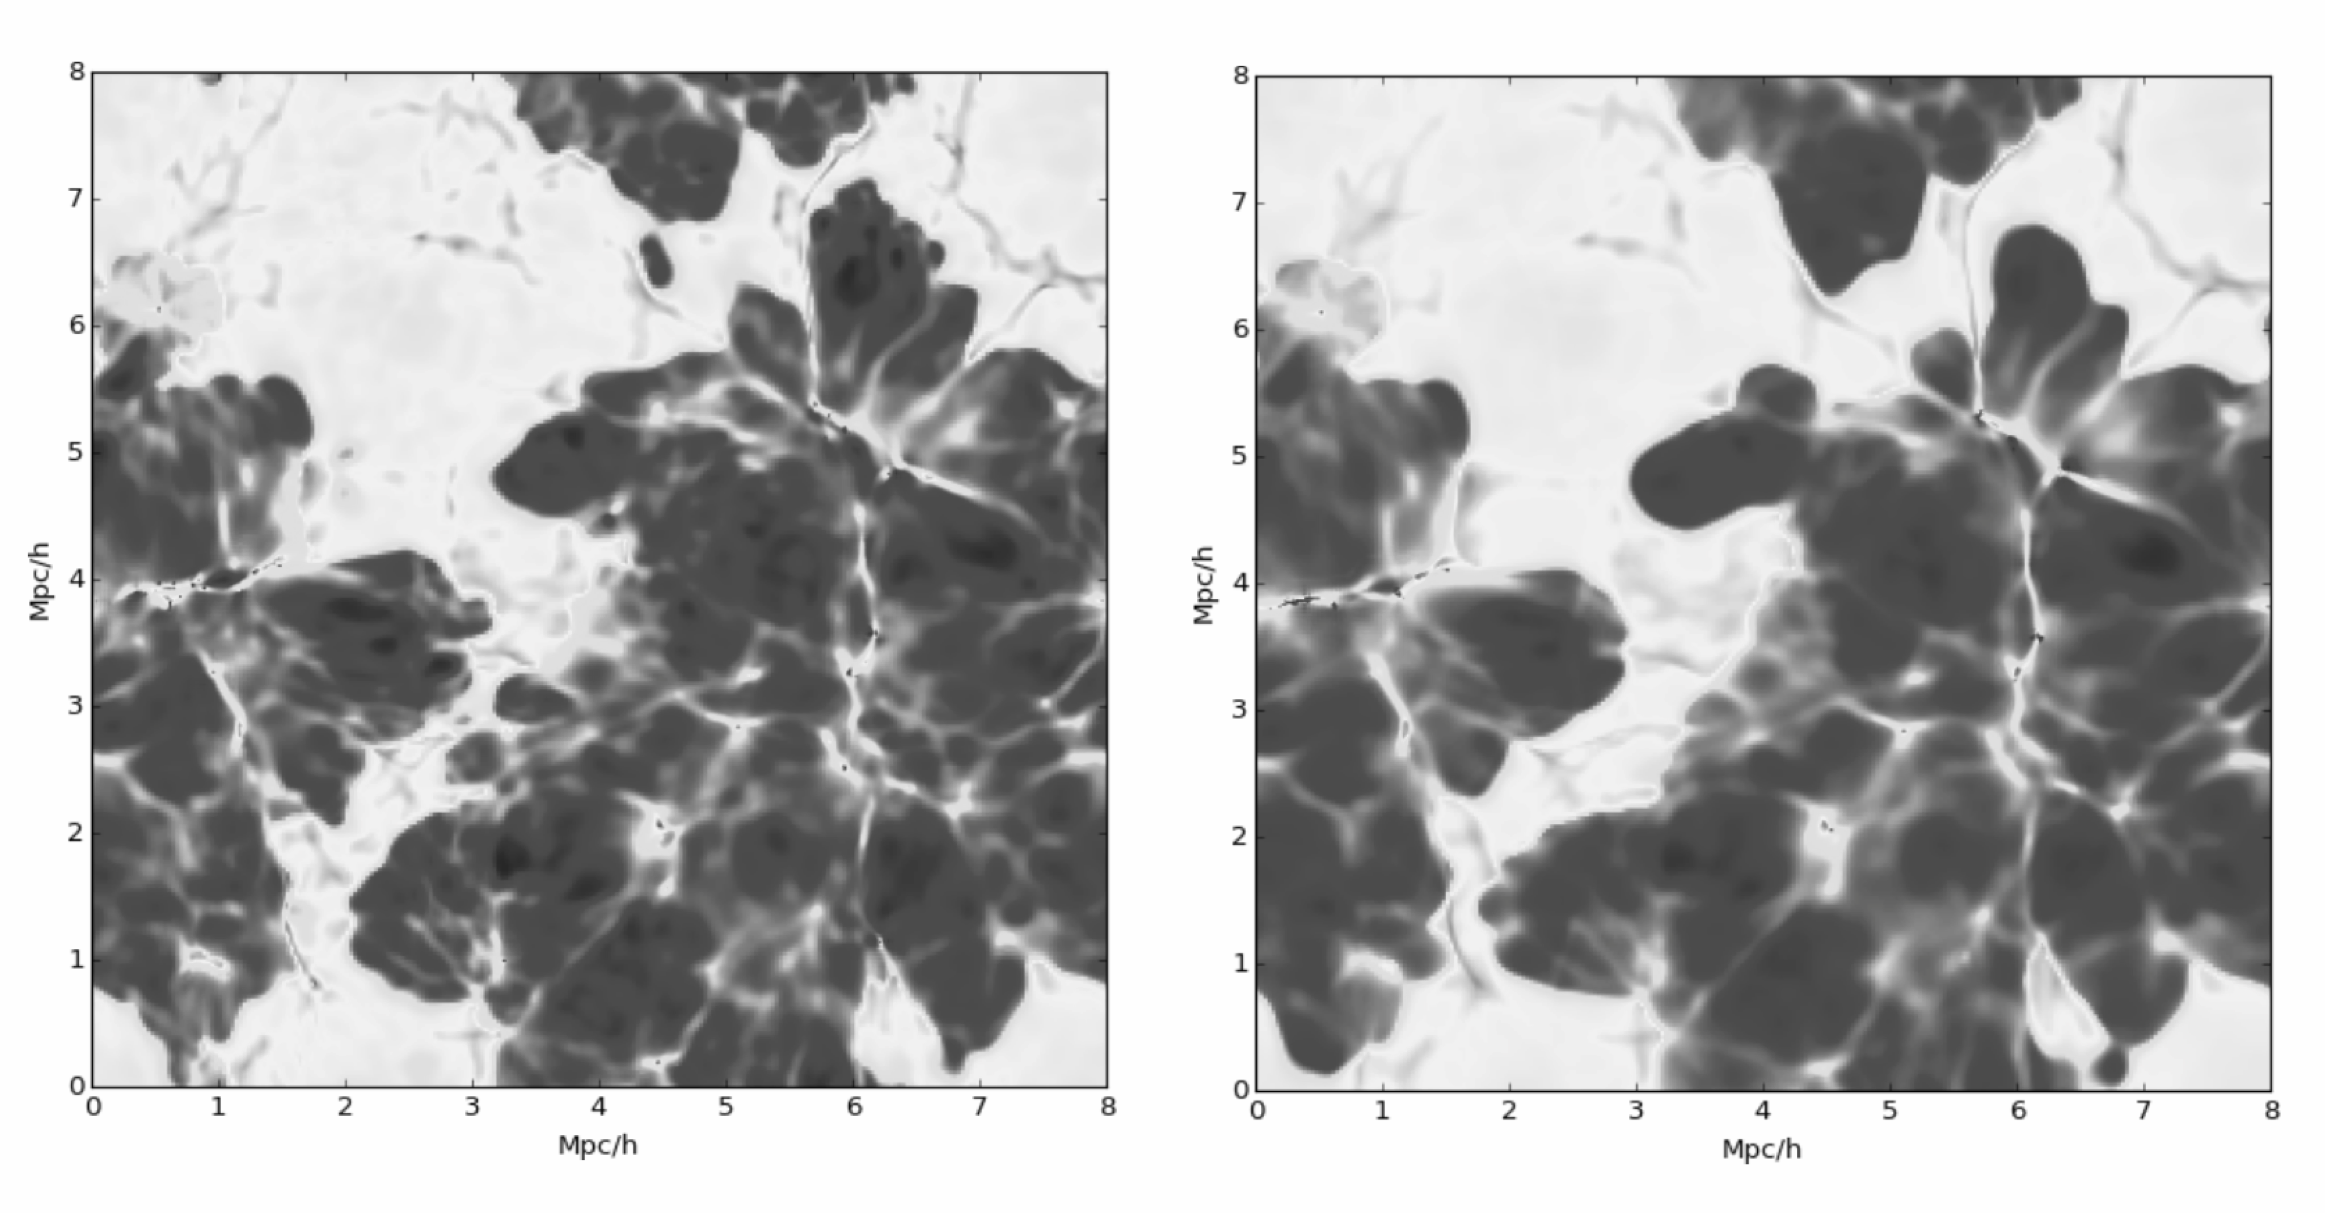
\includegraphics[height=8cm]{figs/wdm.png}
	\caption[Deux simulations de la densité de gaz dans un volume d'Univers de 8 Mpc de côté]{Deux simulations de la densité de gaz dans un volume d'Univers de 8 Mpc de côté, l'un avec de la matière noire froide (à gauche) l'autre avec de la matière noire chaude (à droite). On constate une granulosité plus importante dans le cas de la matière noire froide. Les régions sombres sont ionisées et les claires sont neutres, sans impact pour la discussion ici.} 
	\label{f:wdm}
\end{figure}

On voit aisément que cette taille $\lambda_J$ augmente si la dispersion de vitesse augmente, par conséquent un système chaud créera des structures de grande taille. A l'inverse un système froid pourvu d'une faible dispersion de vitesse, à densité moyenne équivalente, sera capable de produire des structures instables de plus petites taille car la longueur de Jeans est plus faible. De la matière noire froide\index{matière noire froide} fera des petites structures, la matière noire chaude \index{matière noire chaude} plutôt des grandes car elles seules sont assez massives pour contrer la grande dispersion de vitesse. 

C'est une propriété que l'on peut reproduire dans des simulations numériques par exemple (voir Fig. \ref{f:wdm}) et le confrontation des modèles avec les observations permet de mettre une contrainte sur la température de la matière noire. Les résultats sont sans appel : la matière noire doit être froide et non relativiste. En effet le défaut de petites structures dans les modèles de matière noire chaude, en particulier ceux à base de neutrinos\index{neutrino}, ne permettent pas de reproduire l'abondance des galaxies observées autour de nous.

\section{Halos de matière noire et galaxies : difficultés}
\newthought{Les halos de matière noire hébergeraient les galaxies}\index{halo de matière noire} en leur sein. Par conséquent, il apparaît naturel d'extrapoler les prédictions faites sur les populations de halos (invisibles) aux populations de galaxies (visibles). Ceci est d'autant plus tentant que la physique de la matière noire est simple, car uniquement régie par la force de gravitation, tandis que celle devant conduire à la partie visible des galaxies fait intervenir une physique beaucoup plus complexe\sidenote{gravitation, hydrodynamique, chimie, physique stellaire au minimum doivent être ainsi invoquées pour prédire la lumière produite par une galaxie}. Toutefois, le succès des modèles à base de matière noire aux grandes échelles (structure du CMB, distribution de masse dans les amas) ne se transposent pas facilement aux échelles galactiques, et nous allons mentionner ici quelques-uns des défis posés à l'hypothèse de l'existence d'une matière invisible pesante.

\subsection{La fonction de masse des halos}
\begin{figure}[htbp]
	\centering
		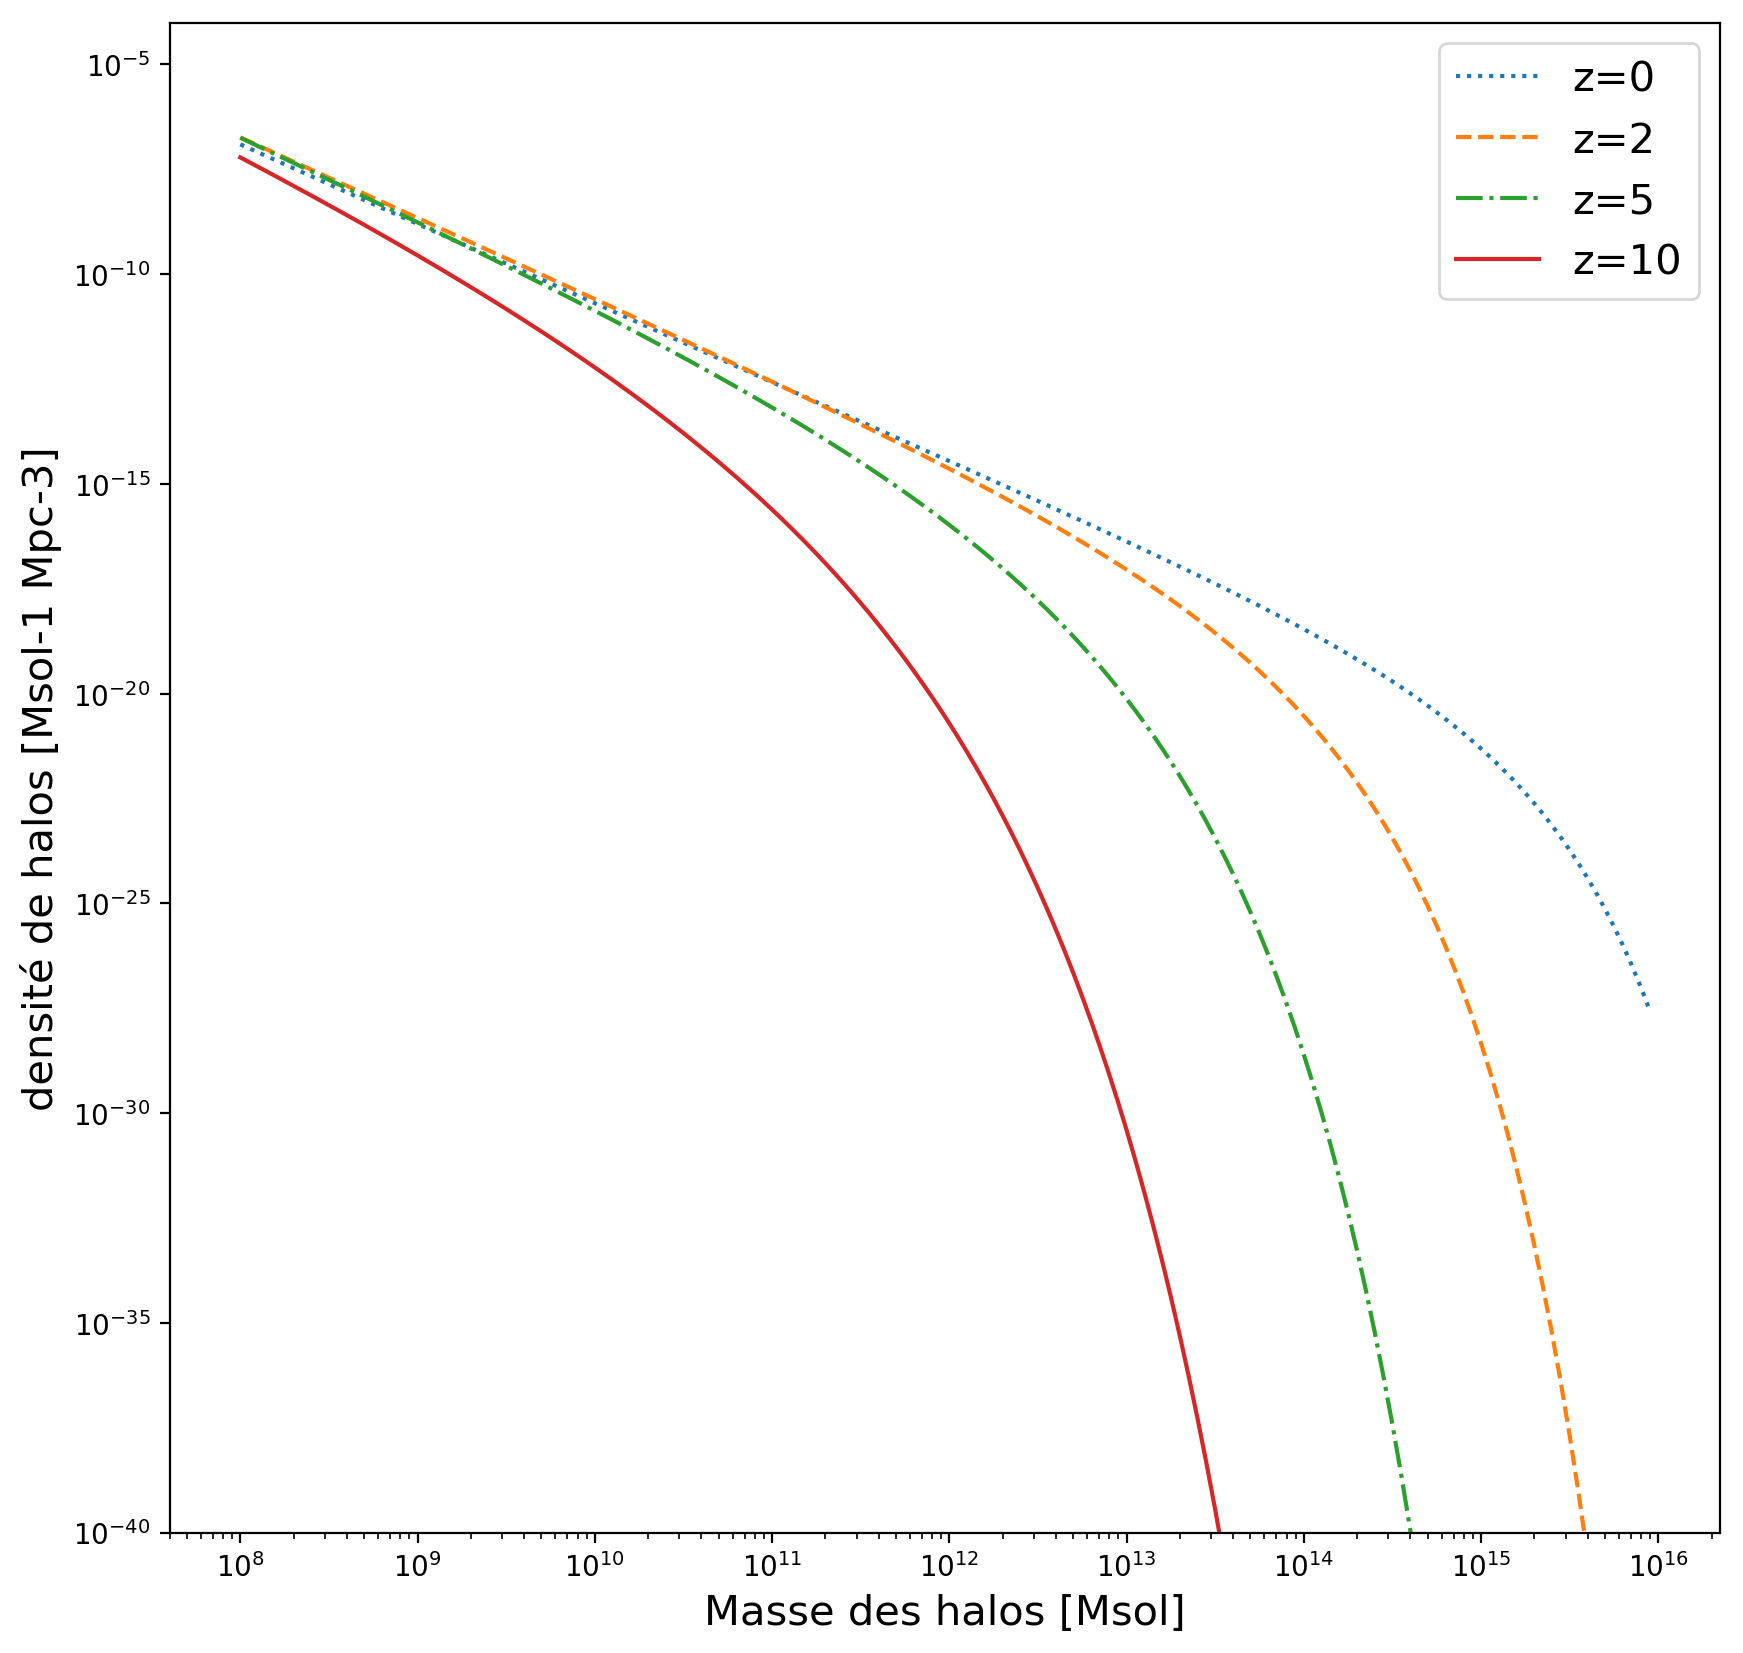
\includegraphics[height=12cm]{figs/hmf.png}
	\caption[La fonction de masse des halos de matière noire pour différents redshifts]{La fonction de masse des halos de matière noire pour différents redshifts. On constate que les halos les plus massifs n'apparaissent que pour des époques tardives: les structures nécessitent du temps pour se mettre en place.} 
	\label{f:hmf}
\end{figure}
L'une des prédictions des modèles de formation des grandes structures\sidenote{voir le chapitre suivant} est la distribution des masses des halos de matière noire. L'obtention de cette distribution est trop complexe pour être abordée ici : elle repose sur la statistique des 'pics' de densités de matière d'amplitude suffisante pour s'effondrer en halos\sidenote{de surdensité environ $\delta_c\sim1.68$, voir le chapitre sur la formation des petites structures}. Cette statistique est définie par son spectre de puissance\index{spectre de puissance}, $P(k)$. La \textit{fonction de masse} dépend de la cosmologie, du type de matière noire, de l'instant considéré et donne le nombre de halos de masse donnée, par unité de volume:
\begin{equation}
dN=f(M,z)dM.
\end{equation}
La fonction de masse\index{fonction de masse des halos} possède une forme caractéristique, décroissante avec la masse considérée : elle indique simplement que les objets peu massifs sont beaucoup plus nombreux que les objets de grandes masses (voir Fig. \ref{f:hmf}). De fait, même si les objets peu massifs ont une contribution individuelle faible au bilan total de masse, en terme de \textit{populations}, ces objets dominent ce bilan. De même son évolution temporelle indique que les objets massifs deviennent de plus en plus nombreux, au détriment relatif des plus légers : c'est le modèle de formation hiérarchique\index{formation hiérarchique} qui est à l'œuvre où les petites structures fusionnent pour en donner de plus grandes au cours du temps. Cela indique également clairement qu'une structure massive de type amas de galaxies\index{amas de galaxies} par exemple, ne peut apparaître que dans un Univers suffisamment évolué : il faut laisser du temps au processus de formation des structures pour qu'il puisse produire des halos lourds. Une autre façon de considérer cette distribution de masse est la mesure de l'échelle typique qu'il faut considérer pour trouver un halo de masse donnée (cf. Fig. \ref{f:L}) : dans ce cas plus un halo est rare, plus l'échelle considérée, plus le volume d'Univers à sonder est important. Par ailleurs, aux époques reculées, on peut constater qu'il est impossible de trouver les halo les plus lourds au sein de l'Univers observable : la raison en est simple, ces objets n'existent pas encore et n'ont pas eu le temps de se former.

\begin{figure}[htbp]
	\centering
		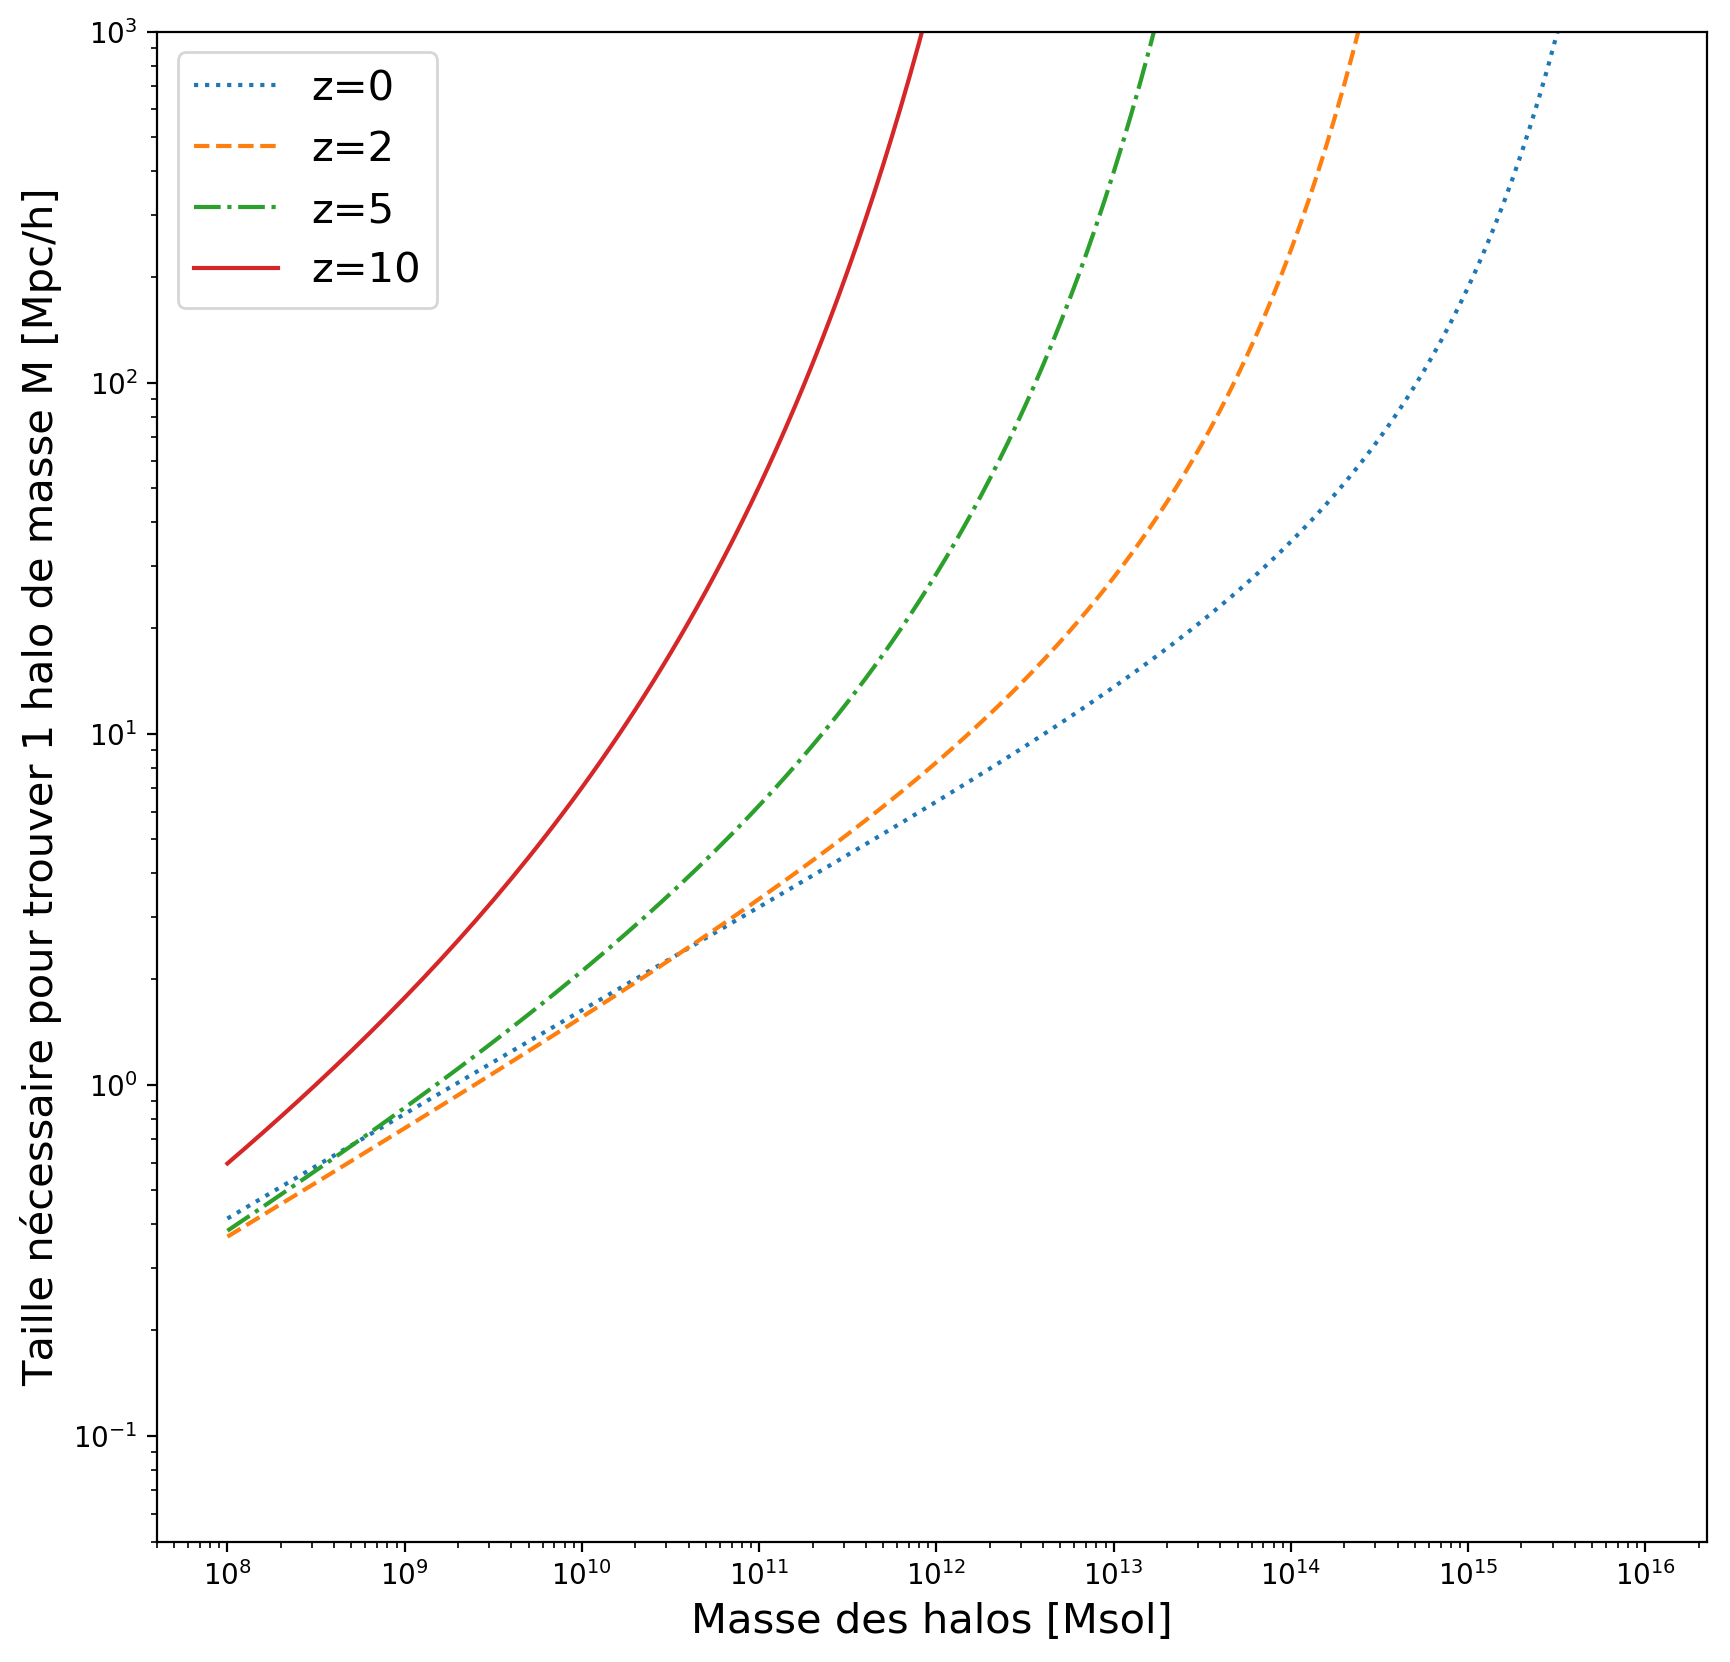
\includegraphics[height=12cm]{figs/L.png}
	\caption[Quelle échelle d'Univers faut-il-sonder pour trouver un halo de masse donnée à une époque donnée?]{Quelle échelle d'Univers faut-il-sonder pour trouver un halo de masse donnée à un redshift donné? Cette courbe indique que plus un halo est léger, plus il est facile de le trouver et plus la taille d'Univers à sonder est petite.} 
	\label{f:L}
\end{figure}

Une première difficulté émerge lorsque l'on compare la distribution des masses des halos avec la distribution des luminosités des galaxies\index{galaxies!fonction de luminosité}. Au premier ordre, il apparaît intuitif de penser que la lumière produite par les galaxies suit la masse des halos sous-jacents : plus un halo est lourd, plus il est mesure de contenir du gaz et plus il est susceptible de contenir des étoiles. Toutefois lorsque l'on compare les distributions de masse des halos et de luminosité, il apparaît que la fonction de luminosité présente un déficit d'objets à la fois aux grandes et aux basses masses \sidenote{La courbure de la fonction est plus prononcée en luminosité qu'en masse}. Cet effet est schématisé dans la figure \ref{f:silkmamon}.
\begin{figure}[htbp]
	\centering
		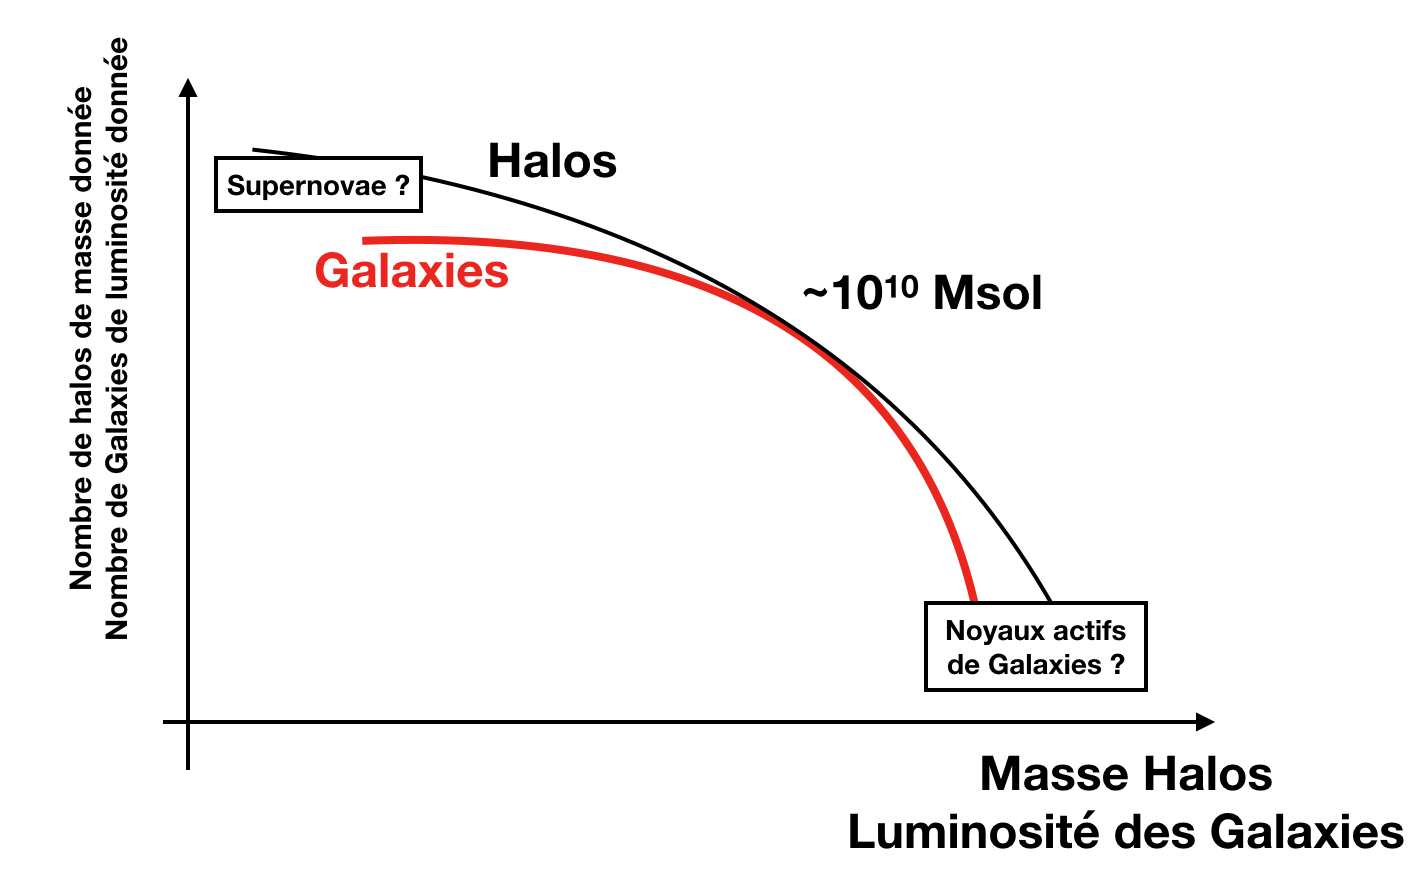
\includegraphics[height=12cm]{figs/SilkMamon.png}
	\caption[Schéma illustrant la différence entre la fonction de masse des halos et la distribution des luminosités des galaxies]{Schéma illustrant la différence entre la fonction de masse des halos et la distribution des luminosités des galaxies. Deux mécanismes sont susceptibles de prévenir la formation d'étoile : les explosions de supernovæ aux faibles masses et les noyaux actifs de galaxie aux grandes masses.  Schéma inspiré de Silk \& Mamon. } 
	\label{f:silkmamon}
\end{figure}
Il faut donc invoquer des mécanismes pour modérer la formation d'étoiles de part et d'autre d'une masse 'pivot' de $10^{10} M_\odot$. Au masses plus faibles que ce pivot, un mécanisme possible est l'injection d'énergie par les supernovæ\index{supernovæ}\sidenote{qui sont des explosions d'étoiles en fin de vie} : celles-ci injectent de l'énergie dans le gaz qui les entoure et le chauffage ou l'éjection de matériau ainsi produits empêchent la formation immédiate d'étoiles de la génération suivante. Aux masses les plus importantes, un mécanisme similaire est envisagé mais cette fois dû aux noyaux actifs de galaxies\index{noyau actif de galaxie}, dont l'énergie produite est lié à l'accrétion de matière sur un trou noir\index{trou noir} supermassif. Dans tous les cas, il faut donc invoquer des processus astrophysiques complexes pour réconcilier la prédiction 'simple' issue de la dynamique de la matière noire avec les propriétés lumineuses des galaxies. Or ces processus sont complexes à appréhender, difficiles à contraindre quantitativement et le modèle de matière noire se trouve ainsi confrontée à un défi particulièrement important à cause de notre compréhension imparfaite de ces phénomènes.

\subsection{Le problème des sous-structures}\index{matière noire!sous-structures}
Une autre difficulté présentée au modèle de halos de matière noire\index{matière noire!halo} est liée aux galaxies satellites présents autour des grandes galaxies. Les objets comme la Voie Lactée\index{Voie Lactée} ou la galaxie d'Andromède\index{galaxie d'Andromède} possède un cortège de galaxies plus légères, dites 'satellites', en orbite autour de la galaxie principale. Au nombre de quelques dizaines par systèmes, ces cortèges posent un défi majeur au modèle de matière noire froide. En effet, ces modèles \sidenote{reposant essentiellement sur des simulations numériques} prédisent des milliers de satellites pour de tels systèmes alors que leur nombre observé se limite à quelques dizaines. Même si la possibilité existe que tous ces objets ne soient pas détectés, il n'en demeure pas moins que l'écart entre théorie et observation est particulièrement frappant dans ce cas (cf. Fig.\ref{f:missing}). Pour expliquer cette différence, il faut à nouveau invoquer des processus qui limitent la création d'étoiles dans la très grande majorité de ces satellites. Ces procédés sont néanmoins extrêmement mal connus et ne permettent pas toujours de résoudre cette tension de façon entièrement satisfaisante.
\begin{figure}[htbp]
	\centering
		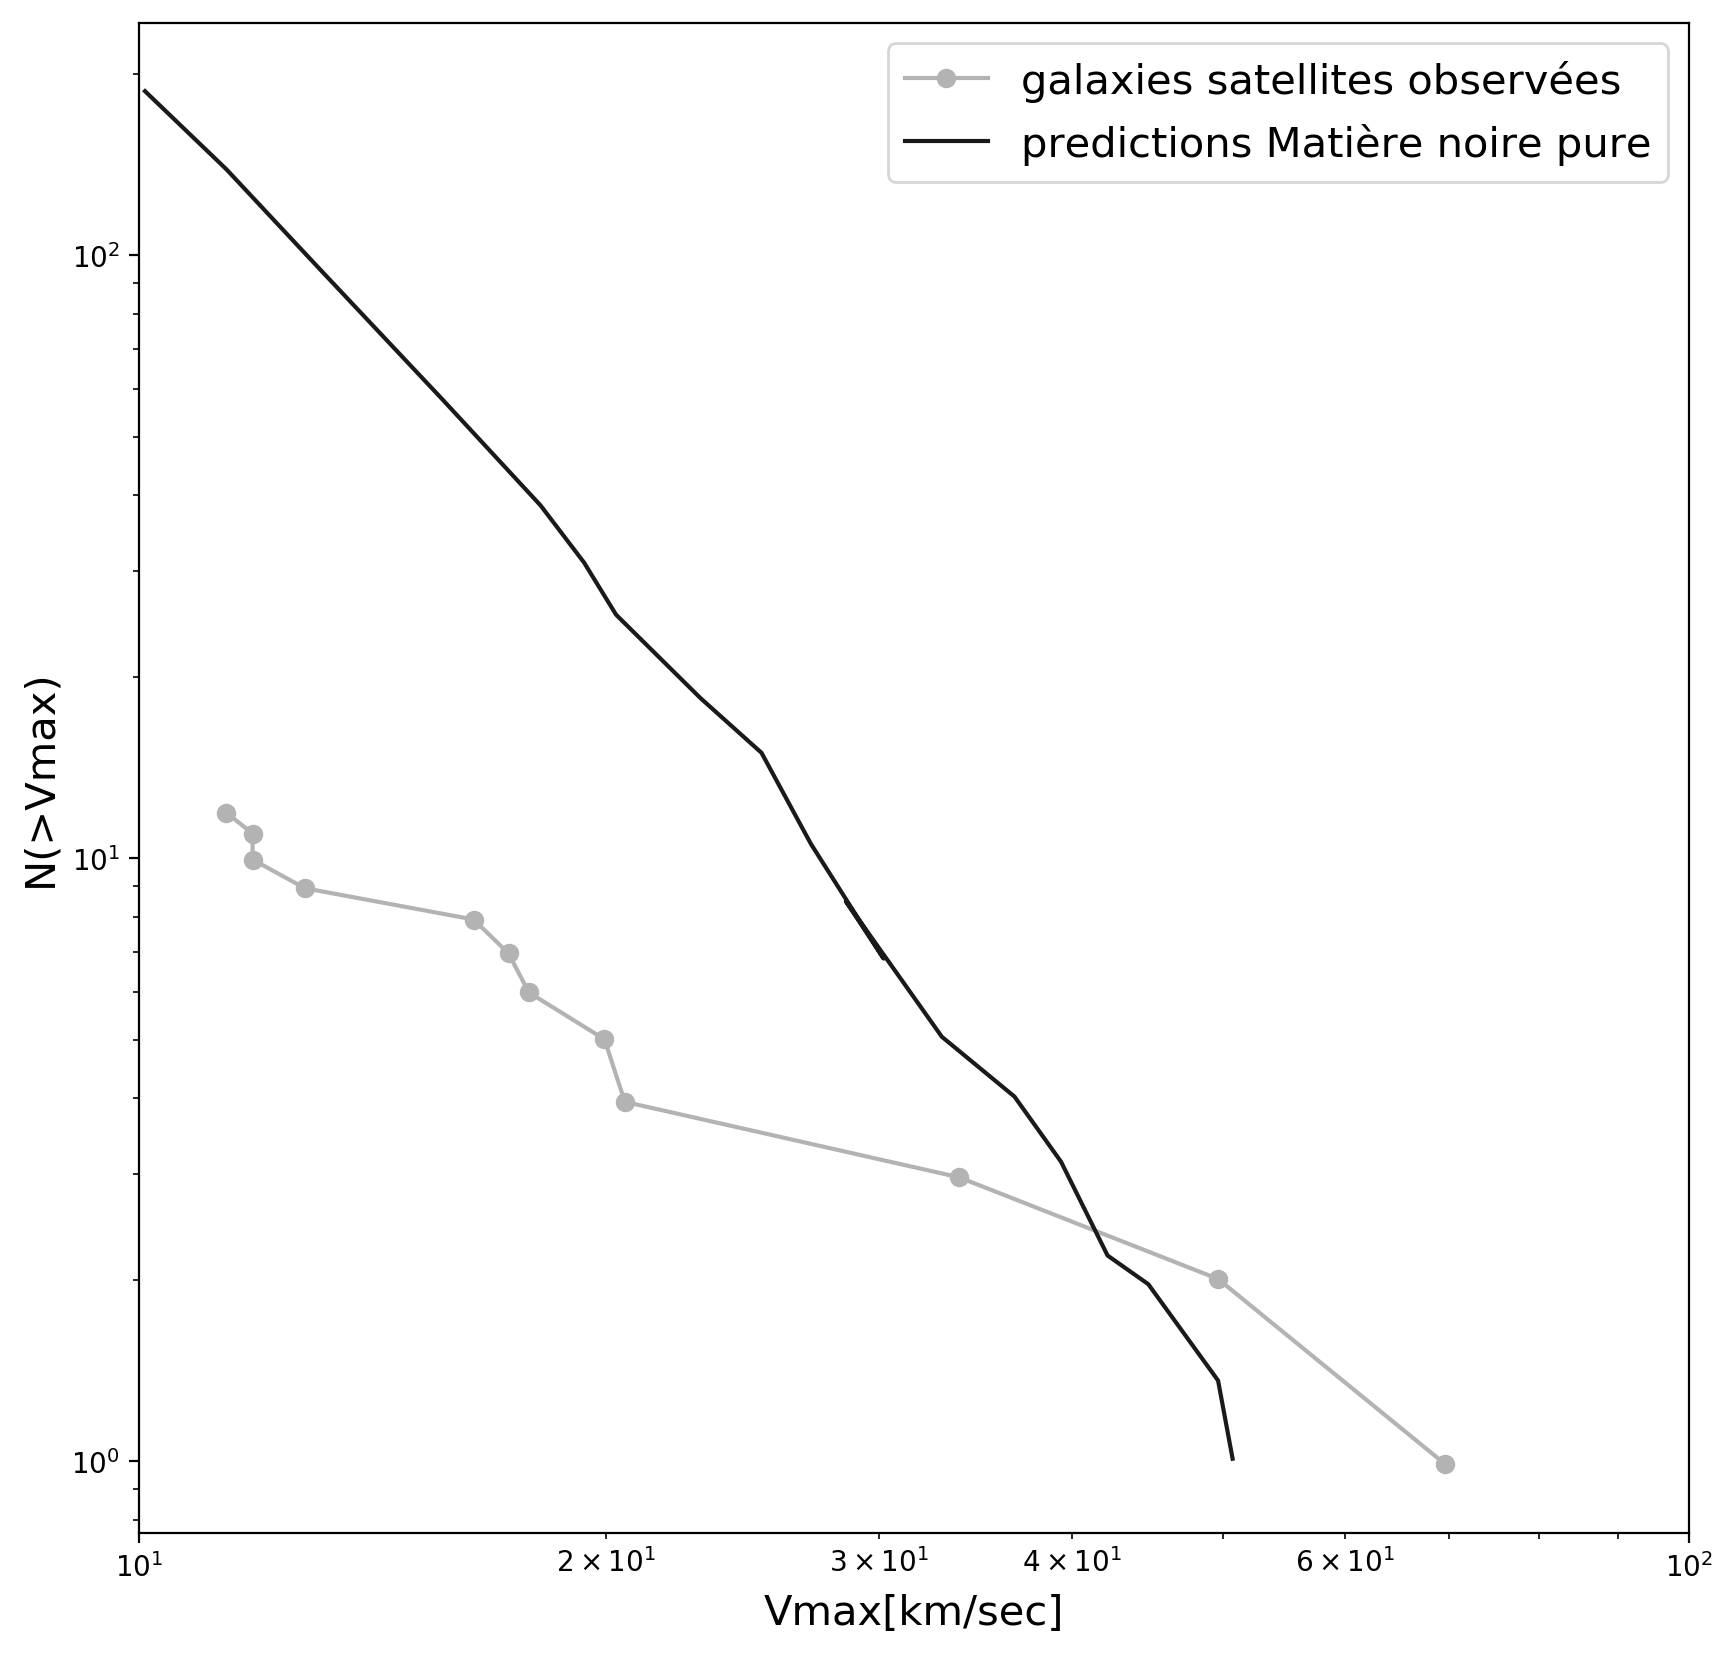
\includegraphics[height=12cm]{figs/missing.png}
	\caption[Distribution du nombre de galaxies satellites de la Voie Lactée]{Distribution du nombre de galaxies satellites de la Voie Lactée possédant une masse supérieure à une masse donnée (la quantité $v_\mathrm{max}$ est une mesure directe de la masse d'un satellite). Les observations sont présentées par les points gris tandis que la prédiction théorique à base de matière noire est donnée par la courbe noire. On constate que les modèles surestiment très largement le nombre observé d'objet. Figure inspirée de Pawlowski et al. (2015). } 
	\label{f:missing}
\end{figure}

\begin{figure}[htbp]
	\centering
		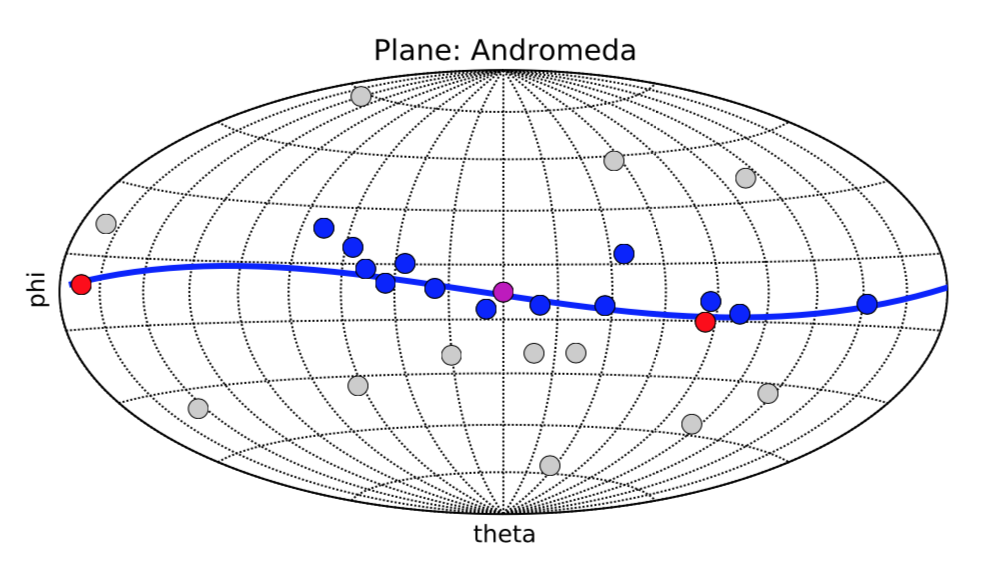
\includegraphics[height=12cm]{figs/planM31.png}
	\caption[Distribution des satellites de la Galaxie d'Andromède]{Distribution des satellites de la Galaxie d'Andromède, vue sur le ciel d'un observateur qui serait placé en son centre. Une quinzaine de satellites sont très proches d'un grand cercle sur le ciel, indiquant que ces objets sont distribués dans un plan.} 
	\label{f:planM31}
\end{figure}

Plus récemment est également apparu le fait que la distribution spatiale de ces satellites\index{galaxies!satellites} n'est pas isotrope mais est organisée sous la forme de grands disques de satellites, fins et en rotation. C'est notamment le cas autour de la Galaxie d'Andromède\index{galaxie d'Andromède} : sur une trentaine d'objets actuellement connus, 15 sont présent dans un grand disque dont 13 en rotation dans le même sens (cf. Fig. \ref{f:planM31}). Or il s'avère que les prédictions à base de matière noire ne parviennent pas à prédire ce type de configuration, tout au moins dans des régimes aussi extrêmes. \sidenote[][-3cm]{ces prédictions reposent sur des simulations et ces simulations ne parviennent pas à reproduire des disques de satellites aussi fins, aussi étendus et dont la cinématique est aussi cohérente.} A nouveau, on peut invoquer des processus qui limitent la formation d'étoile de façon différenciée en fonction de la distance ou de la position de ces satellites pour expliquer cet état de fait \sidenote[][]{le rayonnement provenant de la galaxie d'Andromède elle-même pourrait par exemple éteindre les satellites de façon plus ou moins efficace en fonction de leur distance, expliquant l'étendue des disques.}

Ces 2 problèmes, nombre de satellites ou configuration spatiale de ces derniers, ne sont que deux des exemples les plus critiques auxquels est confronté le modèle des halos de matière noire. Il en existe d'autres et de façon générale il faut invoquer des processus astrophysiques complexes et mal connus de modération de la formation stellaire pour expliquer les différences entre modèle et observation. Pour ces raisons, il est également possible d'envisager qu'il \textit{n'existe pas} de matière noire et il faut donc trouver d'autres raisons pour expliquer par exemple les courbes de rotations plates des galaxies : c'est l'objectif que se fixent par exemple les modèles de gravitation modifiée\sidenote{voir par exemple le modèle phénoménologique MOND (pour \textit{MOdified Newtonian Dynamics}) qui inclut les effets d'une accélération limite dans le régime des faibles champs de gravitation, similaire à l'effet d'une distribution de matière noire}\index{gravitation modifiée}. Toutefois, ces difficultés rencontrés aux échelles galactiques par le modèle de matière noire froide sont à comparer aux succès réels obtenus par ce même modèle aux échelles cosmologiques, pour expliquer la structure du CMB notamment. Pour toutes ces raisons, une grande partie de l'activité actuelle de la communauté vise à tester notre compréhension des processus baryoniques et stellaires pour voir si ils parviennent à réconcilier le modèle de matière noire avec les observations aux échelles galactiques. Cette compréhension est toujours aujourd'hui grandement incomplète.
